\documentclass[12pt,letterpaper]{report}
\newcommand{\prof}[1]{\textbf{\color{red} [#1]}}

\usepackage{natbib}
\usepackage{graphicx}
\usepackage{geometry}
\usepackage{float}
%\usepackage[outdir=./images/]{epstopdf}
%\usepackage{fancyheadings} fancyheadings is obsolete: replaced by fancyhdr. JL
\usepackage{fancyhdr}
\usepackage{afterpage}
\usepackage{graphicx}
\usepackage{amsmath,amssymb,amsbsy}
\usepackage{algorithm}
\usepackage{algpseudocode}
\usepackage{dcolumn,array}
\usepackage{tocloft}
\usepackage{asudis}
\usepackage{booktabs} % For formal tables
\usepackage{color}
\usepackage{mathrsfs}
% \usepackage{unicode-math}
% \setmathfont{XITS Math}
% \setmathfont[version=setB,StylisticSet=1]{XITS Math}


\usepackage{wrapfig}

\usepackage{listings}
\usepackage{color}
\usepackage[labelsep=colon]{caption}

\usepackage{amsmath}
\definecolor{codegreen}{rgb}{0,0.6,0}
\definecolor{codegray}{rgb}{0.5,0.5,0.5}
\definecolor{codepurple}{rgb}{0.58,0,0.82}
\definecolor{backcolour}{rgb}{0.95,0.95,0.92}

\lstdefinestyle{mystyle}{
    backgroundcolor=\color{backcolour},
    commentstyle=\color{codegreen},
    keywordstyle=\color{blue},
    numberstyle=\tiny\color{codegray},
    stringstyle=\color{codepurple},
    basicstyle=\footnotesize,
    breakatwhitespace=false,
    breaklines=true,
    captionpos=b,
    keepspaces=true,
    numbers=left,
    numbersep=5pt,
    showspaces=false,
    showstringspaces=false,
    showtabs=false,
    tabsize=2
}

\lstset{style=mystyle}

\graphicspath{ {images/} }

\begin{document}
%-----------------------front matter
\pagenumbering{roman}
\title{A Framework for Spatial Database Explanations}
\author{Anique Tahir}
\degreeName{Master of Science}
\defensemonth{April}
\gradmonth{May}
\gradyear{2018}
\chair{Mohamed Sarwat, Chair \\ Sharon Hsiao\\ Ross Maciejewski}
\maketitle
\doublespace
\begin{abstract}
In the last few years, there has been a tremendous increase in the use of big data. Most of this data is hard to understand because of its size and dimensions. The importance of this problem can be emphasized by the fact that Big Data Research and Development Initiative was announced by the United States administration in 2012 to address problems faced by the government. Various states and cities in the US gather spatial data about incidents like police calls for service.

When we query large amounts of data, it may lead to a lot of questions. For example, when we look at arithmetic relationships between queries in heterogeneous data, there are a lot of differences. How can we explain what factors account for these differences? This kind of problem can be solved by aggravation: tuples in the database which represents extreme values of our observations, and intervention: tuples in the database which introduce a large change in the observation when removed. We call the predicates which represent these tuples, explanations. Observations by themselves have limited importance. For example, if we observe a large number of taxi trips in a specific area, we might ask the question: Why are there so many trips here? Explanations attempt to answer these kinds of questions over observations.

While aggravation and intervention are designed for non spatial data, we propose a new approach for explaining spatially heterogeneous data. Our approach expands on aggravation and intervention while using spatial partitioning/clustering to improve explanations for spatial data. Our proposed approach was evaluated against real-world taxi dataset as well as synthetic disease outbreak datasets. The approach was found to outperform aggravation in precision and recall while outperforming intervention in precision.
\end{abstract}

% \acknowledgementpage{}
%{Enter your acknowledgement text here}
\tableofcontents
% This puts the word "Page" right justified above everything else.
\addtocontents{toc}{~\hfill Page\par}
% Asking LaTeX for a new page here guarantees that the LOF is on a separate page
% after the TOC ends.
\newpage
% Making the LOT and LOF "parts" rather than chapters gets them indented at
% level -1 according to the chart: top of page 4 of the document at
% ftp://tug.ctan.org/pub/tex-archive/macros/latex/contrib/tocloft/tocloft.pdf

% This gets the headers for the LOT right on the first page.  Subsequent pages
% are handled by the fancyhdr code in the asudis.sty file.
% \addcontentsline{toc}{part}{LIST OF TABLES}
% \listoftables
\addtocontents{lot}{Table~\hfill Page \par}
\newpage
\addcontentsline{toc}{part}{LIST OF FIGURES}
\listoffigures
\addtocontents{lof}{Figure~\hfill Page \par}
\newpage
% \addcontentsline{toc}{part}{LIST OF SYMBOLS}
\clearpage
% \symbolspage{}
% \addcontentsline{toc}{part}{PREFACE}
\clearpage
\addtocontents{toc}{CHAPTER \par}
% \prefacepage{\\Enter content here.}

% This gets the headers for the LOF right on the first page.  Subsequent pages
% are handled by the fancyhdr code in the asudis.sty file.


%-----------------------body
\doublespace
\pagenumbering{arabic}
% \include{chapter0}
\chapter{PROBLEM OVERVIEW}


\label{sec:Intro}
\section{Introduction}

% Motivation
When we analyze data, we might make some observations that pique our curiousity. We might want to explain trends or anomalies in data. Without an automated system, a data analyst has to go through several manual operations to find an explanation. If the size of the data is small, doing so might take a bit of time, but if we are dealing with a large amount of data, it can become a tedious process. Our system is designed to answer questions based on observations over a large amount of data. In the past few years there has been a lot of developments in the area of Big Data.

We can find several examples of decisions being made using big data analysis in everyday situations. Companies like Uber and Facebook handle large amounts of spatial data every day. This data can be used to improve service. UPS is saving millions of gallons of fuel per year by using Big Data Analytics. UPS uses On-Road Integrated Optimization and Navigation system(ORION) to determine the order of delivery, routes, and loading plans \citep{upsarticle}.

Given the tremendous benefits of automated analysis, the motivation for this thesis was to create an automated system to help analysts answer questions about observations. The idea is to create a system which works on spatial data in general. This thesis comes up with a generic system to explain observations on spatial data.

% For example, if we have taxi cab data, we might want to use this data to figure out the best locations for taxi cab stands. Good locations for taxi cab stands can result in less fuel consumption and lower wait times for the customers. A similar case can be made for medical emergencies and hospital locations. Even though, the cost of building a hospital is much higher than that of building a taxi station, the initial cost of building the infrastructure is assuaged over time if the location is beneficial. Companies like

\begin{figure}[ht]
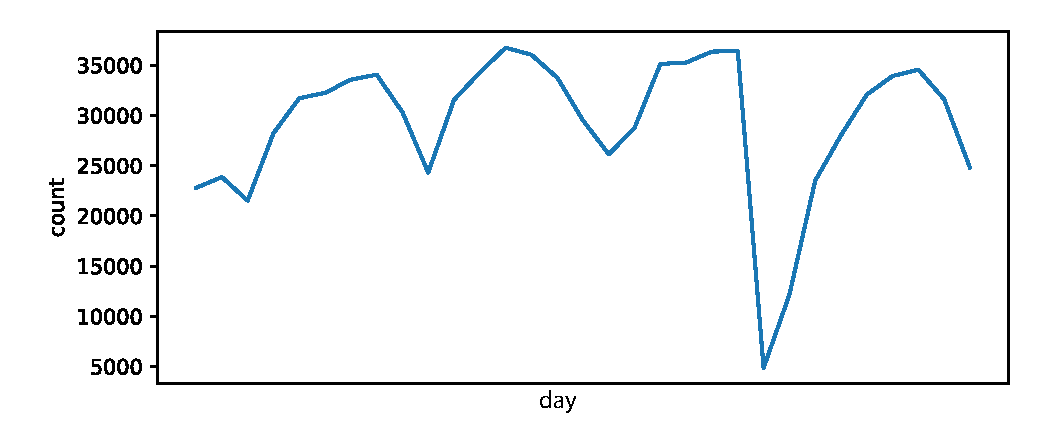
\includegraphics[width=\columnwidth]{yellowdata_count.eps}
\caption{Average number of yellow cab trips against the day for January 2016}
\label{fig:yellowstats}
\end{figure}

The New York City Taxi and Limousine Commission (NYC TLC) regulates yellow cab taxis\citep{taxi2016tlc}. It has licensed around 146,000 distinct drivers. In order to view a demonstration of the database explanation system, we can use this dataset. The Yellow Cab data has several attributes including spatial attributes such as latitude, longitude and non spatial attributes such as tip amount and total amount for each trip. Fig.~\ref{fig:yellowstats} shows the number of yellow cab trips against time for January 2016. The sharp decline in the number of trips in the last quarter of the month is pronounced. One might be inclined to look up the date when the number of trips crashed. In this paper, we look at different approaches to explain these types of observations. In fact, we also look at observations with a spatial dimension.

Whenever we analyze some data, we might be tempted to find out a reason for specific observations. While some data observations might be interesting, in order to make decisions based on these observations, one might find it useful to find an explanation. For example, someone looking to start a business might look at locations in which their specific category of business succeeds. It might be even more beneficial to find out why it prospers in that specific location.

This thesis describes a system that we have created to explain database observations. Our system intends to produce spatial explanations. There are two types of input to our system. One of the inputs is the dataset we want to analyze. The second input is our observation. The observation can be in the form of an aggregate query. Our system uses one of several different solutions to find an explanation depending on what the user wants. The output of our system is an explanation for our system based on predicates.

The explanations produced by our system are formally defined later on in this document. However, it is important to introduce the basic idea so the reader can follow along. In our proposed system, explanations are parts of the data that have a significant effect on what we are observing. For example, if we are observing tips for taxi trips and removing a few tuples from the dataset has a significant effect on the tips, then the few tuples would be considered as an explanation for our observation. Another definition of explanations in our proposed solution involves looking at different parts of the data. For example, if we divide our data into a number of parts, the parts which deviate from the average value of tip percentage are considered as explanations because they introduce the largest differences.

In this thesis we define a taxonomy(Section~\ref{sec:taxonomy}) for observations and explanations.  The observation we made in Fig.\ref{fig:yellowstats} can be considered as a non spatial observation. Its explanation can either be non spatial or spatial. The first class in our taxonomy deals with non spatial explanations for non spatial observations(Section~\ref{sec:nonspatial_nonspatial}). The second class is related to spatial explanations for non spatial observations(Section~\ref{sec:spatial_nonspatial}) while the last class is about spatial explanations for spatial observations. Many geospatial datasets that we encounter contain time as one of the attributes. When we talk about spatial explanations, we do not take time into consideration. Instead, time is considered as a non-spatial attribute.

There are three main approaches to explanation that we study in this thesis. Each approach has been extended to satisfy our taxonomy. Each approach relies on the fact that the observation is an aggregated attribute in our data set while the explanation is a predicate. \textbf{Aggravation}(Section~\ref{sec:aggravation}) is based on the principle that if we consider only the tuples in our database satisfying our explanation predicate, the value of the observation on our modified dataset will be our measure of aggravation\citep{roy2014formal,meliou2014causality}.

In contrast, \textbf{Intervention}(Section~\ref{sec:intervention}) measures the influence of our explanation i.e. what will be the value of our observation when all the tuples satisfying our explanation predicate are removed\citep{roy2014formal}. We also extend Intervention to introduce \textbf{Hierarchical Intervention}(Section~\ref{sec:hei_intervention}). This approach measures the value of intervention when the explanation consists of a cluster of spatial polygons in our explanation predicate.

Finally, \textbf{Salient Features}(Section~\ref{sec:salient_features}) can be used to find explanations\citep{chirigati2016data}. Each salient feature encapsulates a polygon where an attribute in the dataset is pronounced. The correlation between a salient feature of the observation and the salient feature of the explanation can give us possible explanations.

Each approach has its own set of advantages and disadvantages. While one approach might give us very specific explanations that show a textbook example of our observation, another might give us an explanation which is hard to see in the context of the observation but has a large overall impact on it. One of the objectives of this paper is to compare which approach is suitable considering its context.

We implemented(Section~\ref{sec:implementation}) these approaches, including hierarchical intervention using distributed data frameworks\citep{borthakur2007hadoop,dean2008mapreduce,shanahan2015large,zaharia2016apache}. We made optimizations in our implementation to make sure our approach is orders of magnitude faster than the naive approach. The implementation of salient features was used from the Data Polygamy framework \citep{chirigati2016data}.
\newpage
In order to compare each approach, we defined a few evaluation metrics. The \textbf{Intensity}(Section~\ref{sec:intensity}) metric measures how relevant each explanation is to the observation. To be more specific, it measures the value of the observation for the top explanations for each approach. The \textbf{Influence}(Section~\ref{sec:influence}) metric measures the observation when the top explanation is removed from the data. We also compare the speed(Section~\ref{sec:speed}) of our implementations of each approach.

\section{Related Work}
There has previously been some work related to database explanations. Most of this work revolves around the notion of causality. There is existing work in the field of Artificial Intelligence by \cite{zhang2002discovering} which expresses relationships between different attributes in a dataset as conditional probabilities. Based on the conditional probability each tuple is given a set of binary rankings.

The work by \cite{meliou2010causality} is a survey which looks at causality from the perspective of a database problem. Traditionally, work on causality from the database perspective mainly deals with provenance i.e. events which occurred chronologically. This solution, however, only works with databases with timestamps. This paper also looks at the degree of responsibility which is defined as the number of tuples which have to be removed to change a binary observation. An example of a binary observation is winning and losing an election for instance. If a candidate wins by a high margin, each tuple has a lower degree of responsibility. On the other hand a close victory for a candidate increases each voters degree of responsibility.

The paper by \cite{meliou2014causality} is a survey of work in causality and explanations in both the Artificial Intelligence and Database communities. The take away from this survey is that AI problems tend to have a bigger causal network while database problems tend to have more variables.

There has also been a lot of work on correlation which shares some common ground with the work on explanations. One interesting recent work on the subject is the Data Polygamy framework\citep{chirigati2016data}. This framework is designed to find the correlation between a corpus of datasets. It uses the peaks and troughs of the data to calculate \textit{salient features} \citep{dunn1986applied}. The positive and negative correlation between these salient features can be used to decide whether dataset are related\citep{su2014supporting}. The objective of our system is a bit different from finding corelations. There are a number of different factors which can effect observations. Correlation might be one of these attributes in certain cases but if we ignore other criteria such as selectivity then we might get results which do not have a significant impact. E.g. if two attributes are highly corelated in a certain spatial cluster but the selectivity of the cluster is small, it would lead to a low impact on the observation.

There has also been work related to why not explanations in databases. The work by \citep{ten2015high} looks at the question of why some tuples are missing from database results. This paper uses the assumption that the relationship between tuples is defined in the form of an ontology. The paper uses the relationship between the ontology for a schema and the ontology for an instance of the schema to judge whether an explanation exists. The ontologies that are used can be created manually or automatically. Using provenance \citep{cheney2009provenance} can help in creating ontologies.

Our solution mainly builds upon work by \cite{roy2014formal} which outlines a formal approach to explain data. The main solutions outlined in that work are Aggravation and Intervention. The work by \cite{roy2014formal} is designed to work with non spatial datasets. One of the main points of the paper is that their approach works on a dataset which can span several tables related by primary and foreign keys. While the approach outlined by \cite{roy2014formal} is great for non spatial data, it does not translate well in the spatial domain. This approach develops on previous work in causality and influence. It also resembles data mining concepts related to association rule mining\citep{agarwal1994fast,tan2006introduction}. In association rule mining sets of attributes that occur together are assigned a support and confidence. The support measures the frequency of occurrence of a set of attributes while confidence measures how frequently an attribute occurs with another set of attributes. The work by \cite{koperski1995discovery} looks at association rule mining in a spatial context. Given a set of spatial relationships, it applies association rule mining to find relationships that frequently occur together. There is a difference between association rule mining and our prosposed approach. First of all, our proposed approach uses a user defined observation. Secondly, in our approach we are not looking at the associations but rather at the effect of removing or filtering pieces of data. A high association between predicates does not necessarily mean that removing them will significantly effect the observation.

Spatial Analysis is very popular in GeoScience and GeoInformatics. Regression techniques can be used to explain data\citep{dunn1986applied,cleveland1988locally}. The idea behind regression techniques is to express an attribute that we are interested in as a dependent variable. This dependent variable can then be expressed in the form of parametric equation involving other attributes in the dataset as independent variables. An example of a loss function for this kind of regression is Ordinary Least Squares(OLS)\citep{dismuke2006ordinary}. The user of this system decides a dependent variable and a set of explanation variables. The resulting equation has coefficients assigned to each explanatory variable as well as a bias term. This results in a curve fitting problem. The curve fitting problem is solved using regression i.e. the coefficient terms and the bias are iteratively adjusted until the sum of squared error between the predicted curve and the ground truth results in a minimum value. Regression techniques are widely used for spatial data analysis. However, they depend on predefined spatial partitioning and look at the data as a whole rather than looking at it from the perspective of a user defined observation compared to our solution.

Geographically Weighted Regression(GWR) expands on OLS regression for geospatial data\citep{brunsdon1998geographically,charlton2009geographically}. GWR tries to use the regression equation for each feature in the dataset. It uses the idea that spatially co-located points contribute more to each other by using a spatially aware kernel function. A kernel function like a Gaussian, for example, gives more weight to nearby points than to points which are far apart.

Besides work related to explanation, there has been a lot of research in the area of spatial correlation. Much of the work in this area extends from multiple old works by Getis\citep{getis1991spatial,ord1995local,getis1996local,getis2002comparative,getis2007reflections}. The Getis Ord statistic \citep{ord1995local} for example is useful in showing us areas with high local spatial associations. The Moran's I statistic is useful for measuring the spatial heterogeneity of the data\citep{assuncao1999new,zhang2008use}. Moran's I is useful in hot spot analysis which can be viewed as a step in the way of finding explanations.

\section{Contributions}

In this paper we extend several approaches and compare them. There are three major contributions in this thesis:
\begin{itemize}

\item We extend aggravation and intervention for spatial explanations/observations. Aggravation and Intervention techniques in literature are designed for giving non spatial explanations for non spatial observation. When we look at spatially heterogeneous data, the spatial context has impact on the value of the explanations.

\item We extend the use of salient features to give spatial explanations for simple observations based on attributes. Salient Features can be used to compare the correlation between attributes between multiple datasets. However, we re purpose the use of salient features for explanations. We use the salient features for attributes in the same dataset to form explanations.
\item We introduce a new approach: Hierarchical Intervention. This approach uses spatial partitioning/clustering. We find that there is a difference between explanations for spatially heterogeneous data for different dimensions of spatial explanations. Therefore, we propose a new approach which uses a spatial hierarchy. This accounts for explanations for multiple dimensions of the data.

\item We introduce a method to balance influence and intensity to give better explanations. Influence and Intensity measure the global and local impact of an explanation, respectively. We acknowledge that the user of our system can have a non binary preference for either. We construct our system in a way that it produces explanations as a linear relationship between influence and intensity.

\item We introduce an automated system for giving explanations based on our findings. The system that we have defined has a lot of parameters. It requires observations, coefficients, arithmetic relationships and selectivities as parameters. We have designed a Web based User Interface to help a user with little knowledge of the system to get explanations for their observations.
\end{itemize}

% The approaches that we mention in his paper borrow from previous work on explanation and correlation. We have extended existing frameworks to work on our specific taxonomy. Aggravation(Section~\ref{sec:aggravation}) and Intervention(Section~\ref{sec:intervention}), for instance, are approaches which are originally designed to work in a non spatial context. They provide explanations in the form predicates over attributes. If we have a dataset with latitude and longitude as the spatial attributes, they may provide explanation in terms of just a latitude or longitude as separate continuous attributes. They might even provide explanations with no spatial attributes at all. Another drawback of using these approaches with spatial data is that they function without any knowledge of spatial locality.
%
% We highlight a new approach called hierarchical intervention (Section~\ref{sec:hei_intervention}). This approach intends to use clusters of spatially co located points or polygons in an attempt to come up with better explanations. As the name suggests, this approach borrows from the intervention approach. It uses spatial partitioning to improve spatial explanations.
%
% Another contribution of this paper is outlining a method for using salient features for explanations. The salient features approach is originally intended to work for correlation between datasets. Our extension of this approach intends to use it for the purpose of explanations. Extending salient features for explanation rather than correlation involves some additional step of work while discarding parts of the previous work which relates specifically to correlation. The original work uses salient features to compare multiple datasets and rank the most correlated datasets. Our usage of salient features is intended to explain only a single dataset with multiple attributes. Even if two attributes of a dataset are highly correlated, it may or may not rank the two attributes in the top explanations depending on the observation.

One of the contributions of this thesis is to compare the different approaches. In order for us to compare different things, we need to do so on the basis of a common standard. The different solutions to the explanation problem are structurally very different from each other. As previously mentioned, some of them are originally not designed to handle spatial data. We have designed a common taxonomy to compare all these different solutions. On top of designing this taxonomy, our extension of each approach is designed to make sure each solution adheres to the taxonomy. Even though, this still leaves room for differences between each solution, it gives us room for comparison.

We also define a number of evaluation metrics and an approach which uses them to come up with better explanations.

% \section{Document Outline}
%
% This section is intended to  give an outline of the remaining document:
%
%
% Chapter~\ref{chp:prelims} goes over the various nomenclature, tools, and techniques that we use throughout the paper.
%
% Chapter~\ref{chp:architecture} goes over the taxonomy for our observation/explanation system. It goes over the different kinds of observations and explanations. It also goes over different explanation techniques in literature, how they compare, and their significance for different contexts.
%
% Chapter~\ref{chp:proposed} deals with outlining our proposed system. It goes over an outline of our proposed system. Gives an explanation of various clustering schemes that we use. We also go into the implementation details of our system in this chapter. Finally, we go over the user interface that we have designed to interact with our system.
%
% Chapter~\ref{chp:eval} gives details about the various experiments we performed as well as the evaluation for our proposed system.
%
% Chapter~\ref{chp:concl} gives concluding remarks about this work as well as ideas about future work.

\chapter{Preliminaries}
\label{chp:prelims}
In order to understand the system. The reader needs to understand a few concepts related to Data Mining and Databases. This chapter attempts to give a brief overview of the underlying concepts needed to understand the system.

\section{Star Schema}
Our system has the underlying assumption that the data that will be used to generate explanations is the Fact Table for a Star schema\citep{giovinazzo2000object,adamson2010star}. To understand the Fact Table, it is important to understand the structure of the Star Schema. A traditional relational database system contains a set of tables related by primary and foreign keys. For instance, We may take the example if student taking courses. The students and classes can be represented in separate tables. One student can take multiple courses and a course can have multiple students. This is an example of a many-to-many relationship.
In order to represent this data in a relational database, the course table and the students table need to have a primary and foreign key. Another way of storing this data without primary and foreign keys is to save all students information against all course information. Tables.~\ref{tbl:fact} and ~\ref{tbl:payment_type} show some dummy data to illustrate our example.

The illustrated example has a normalized schema\citep{beeri1988sophisticate}. Table~\ref{tbl:fact} can be considered as the central part of the schema because it contains the foreign key to the $payment_type$ table.



\begin{center}
  \begin{tabular}{ | l | c | }
    \hline
    \textbf{PaymentTypeId} & \textbf{Name} \\ \hline
    1 & Credit Card  \\ \hline
    2 & Cash  \\ \hline
    3 & No Charge  \\
    \hline
  \end{tabular}
\end{center}
\captionof{table}{Payment Type Table}
\label{tbl:payment_type}

% \begin{center}
%   \begin{tabular}{ | l | c | r | }
%     \hline
%     \textbf{StudentId} & \textbf{Name} & \textbf{Grade} \\ \hline
%     1 & John Doe & 3.2 \\ \hline
%     2 & Alice & 3.3 \\ \hline
%     3 & Bob & 3.8 \\
%     \hline
%   \end{tabular}
% \end{center}
% \captionof{table}{Students Table}
% \label{tbl:student}

\begin{center}
  \begin{tabular}{ | l | l | c | l | }
    \hline
    \textbf{pickup\_lat} & \textbf{pickup\_lng} & \textbf{PaymentTypeId} & \textbf{tip\_percentage} \\ \hline
    34.4 & -74.2 & 1 & 15.3 \\ \hline
    34.6 & -74.1 & 1 & 10.2 \\ \hline
    34.6 & -74.3 & 1 & 9.8 \\ \hline
    34.8 & -74.6 & 2 & 11.2 \\ \hline
    34.6 & -74.3 & 1 & 10.7 \\ \hline
    34.9 & -74.1 & 3 & 0.0 \\
    \hline
  \end{tabular}
\end{center}
\captionof{table}{Fact Table}
\label{tbl:fact}

This type of schema where the there is a central table consisting of facts while the remaining tables contain the meta data is called a star schema. The central table is called the Fact Table, whereas, the tables containing the meta data are called the Dimension Tables.

\section{Observations}
\begin{figure}[ht]
  \begin{center}
  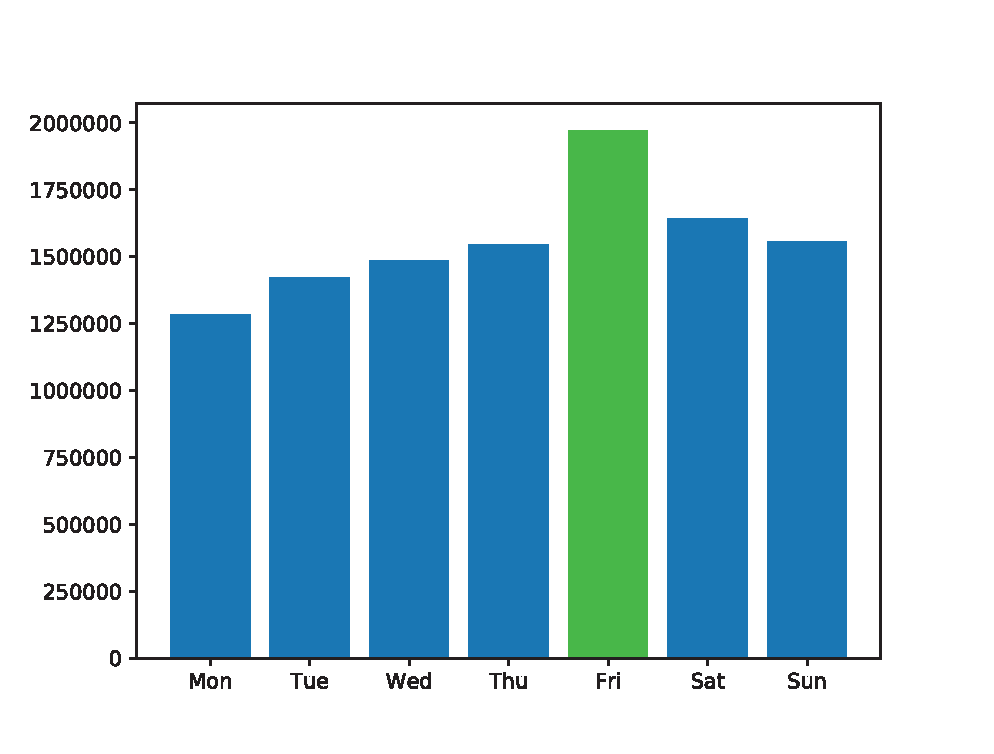
\includegraphics[width=0.5\columnwidth]{observationexample}
  \end{center}

  \caption{An histogram showing an example observation}
  \label{fig:observation_example}
\end{figure}
Observations are features in the data that the user wants to explain. Observations are defined as arithmetic expressions over a set of aggregate queries. Let $F$ be the fact table in our star schema dataset. In the course of this document, we will be using relational algebra expressions defined by \cite{elmasri2011fundamentals} for aggregate expressions. Thus, the $\mathscr{F}$ symbol represents an aggregate function. An aggregate query is defined as:
$$_A\mathscr{F}_B(D), A \in F$$
$B$ is an aggregate function. An examples of an aggregate function include SUM, COUNT and AVERAGE.
We use SQL to construct an example for an observation. Queries~\ref{qry:aggregateexample1} and \ref{qry:aggregateexample2} show examples of aggregate queries.

Observations made on data can also be represented on histograms. Fig.~\ref{fig:observation_example} shows an example of an observation. The green bar on the histogram represents an aggregate query where where the day is Friday.

\renewcommand{\lstlistingname}{Query}% Listing -> Algorithm
\begin{lstlisting}[language=SQL, caption=Aggregate Query for average tip percentage with credit cards, label=qry:aggregateexample1]
SELECT AVG(trip_percentage) FROM
FROM nyc_data
WHERE payment_type = 1
\end{lstlisting}

\renewcommand{\lstlistingname}{Query}% Listing -> Algorithm
\begin{lstlisting}[language=SQL, caption=Aggregate Query for average tip percentage with cash, label=qry:aggregateexample2]
SELECT AVG(trip_percentage) FROM
FROM nyc_data
WHERE payment_type = 2
\end{lstlisting}

Using these aggregate queries we may form an observation based on the ratio of tip percentage with credit card against tip percentage with cash.
$$observation = \frac{\textnormal{Query.~\ref{qry:aggregateexample1}}}{\textnormal{Query.~\ref{qry:aggregateexample2}}}$$


\section{Explanations}
We represent explanations as a predicate. A predicate is a conditional statement which results in a boolean value. We go into more details for the formal definition of different kinds of explanations in Section~\ref{sec:taxonomy}. If we consider Queries~\ref{qry:aggregateexample1} and \ref{qry:aggregateexample2} as an example. The explanation would be in the form of a predicate:
$$tip\_percentage = 15.3$$

Let $D$ be our solution space. We can define our predicate to be the function $P$. Our explanation can now be formally defined as:

\begin{equation}
x|P(x):=
    \begin{cases}
      \text{true}, & \text{if}\ x \in D \\
      \text{false}, & \text{otherwise}
    \end{cases}
\end{equation}

Note that $P$ is an open ended function. In the case of spatial explanations it can take the form of a spatial function like $ST_CONTAINS$ i.e. whether a polygon contains a point.

\section{K-Folds Cross Validation}
K Folds cross validation is a technique for data evaluation\citep{kohavi1995study,refaeilzadeh2009cross}. The data is divided into $k$ parts. One of the parts is used as a training set and the remaining parts are used as test sets. The purpose of the training set is to model the data. Once we have a model, we can use it to classify and/or predict the unseen data. The test set is used to evaluate how well the model was trained.

\section{Precision and Recall}
Precision and Recall are methods for evaluation\citep{olson2008advanced,powers2011evaluation}. Whenever we classify data we may have true positives, false positive, true negative and false negatives. Precision is defined as:
$$precision = \frac{\textnormal{true positives}}{\textnormal{false positives} + \textnormal{true positives}}$$

Recall is defined as:
$$recall = \frac{\textnormal{true positives}}{\textnormal{true positives} + \textnormal{false negatives}}$$

\section{Distributed Processing Frameworks}
Map Reduce\citep{dean2008mapreduce} is a framework for data processing which is designed with taking distributed and parallel computation into perspective. There are three main operations in a mapreduce process: map, shuffle and reduce. The map operation assigns a key to each element, and performs any necessary transformations. The shuffle operation relocates the elements such that elements with the same key are nearby(since they are going to need each other in calculations). The reduce step performs calculation on each element with the same key and returns the output.

Spark\citep{shanahan2015large,zaharia2016apache} is a distributed and parallel processing framework. The Spark uses a directed acyclic graph to perform calculations. Since the DAG created by Spark can have a lot of common nodes between tasks, the computational complexity of the operation is reduced compared to MapReduce.

Geospark~\citep{yu2015geospark} is a framework for performing several spatial operations on data in Apache Spark. It also has a component which helps in data visualizations\citep{yu2018src}.

\section{Front End Visualization Tools}
React\citep{reactjs} is a front end framework which originated in Facebook. React framework allows interfaces to be designed using Components. Each components have properties and a state. A component can have subcomponents. This makes it simpler to design interfaces which show consistent data across components. Some of the charts included in the interface make use of the eCharts library\citep{echarts}.

MapBox\citep{mapbox} is a library for displaying maps. The maps provided by mapbox consists of tiles and vectors. Each tile represents a cube of the map while vectors are shapes which represent roads, buildings etc. Deck.gl\citep{deckgl} is a library for creating an overlay on top of the map. Examples of overlays include scatterplots, cartograms etc. Matplotlib was also used for static plots for evaluation\citep{hunter2007matplotlib}.

\chapter{System Architecture}
\label{chp:architecture}
\section{Taxonomy}
\label{sec:taxonomy}
We define a taxonomy for observations and explanations. This taxonomy will help us standardize different approaches to explanation. It will also help us compare these approaches against each other. Our observation/explanation standard is based on the assumption that observations take the form of a query, whereas, explanations take the form of a predicate. Let $D$ be the dataset that we are interested in. Let $A_D$ be a set of attributes of $D$. Let $V_a$ represent the set of values for in $D$ for attribute $a$ where $\{\neg \emptyset,\emptyset\} \subset V_a$. Then we can define our candidate explanation $\phi$ as $$\phi \models \wedge_{i,j} {(i=j)}$$ where $i \in A_D, j \in V_i $

The observation is simply just an aggregate query on $D$. Each approach returns a set of candidate explanations and there is a value associated with each candidate explanation which measures its score. We define the scoring function for each approach in its respective section in the document.

\subsection{Non spatial explanation for non spatial observations}
\label{sec:nonspatial_nonspatial}

Non spatial observations are aggregate queries on $D$. These queries can take any form. Non spatial explanations are candidate explanations based purely on non spatial attributes of the data. Let $S$ be the spatial attributes in $D$. Our candidate explanation can be defined as
$$\phi \models \wedge_{i,j} {(i=j)}$$
where $i \in A_D, i \notin S, j \in V_i$

We can look at an example of non spatial explanations for non spatial observations by looking at the NYC TLC data for Yellow Cab. There are several attributes which are continuous e.g. tip amount, trip distance, and fare amount. A month of taxi trip data consists of 10 million tuples. This means that if we find all possible combinations of attribute values, it can exceed over a million. Instead each of the approaches we discuss tries to simplify how the explanations are calculated. For instance, salient features use crests and troughs in the value of an attribute over time. Fig.~\ref{fig:yellowstats} shows the average number of taxi trips per day for one month. If we consider twenty thousand trips as an upper bound, we only get part of the curve which we call a salient feature(Section~\ref{sec:salient_features}). We can use this salient feature for our explanations. The upper bound in the case of salient features is either user defined, or automatically generated. We discuss the details of the salient features implementation in Section~\ref{sec:salient_features}


\subsection{Spatial explanations for non spatial observations}
\label{sec:spatial_nonspatial}

Spatial explanations take the spatial attributes of the data into consideration. In contrast to non spatial explanations, the candidate explanations for spatial explanations contain polygons. Since we base our method on the assumption that important tuples are spatially co-located, points which fall inside these polyons form a candidate explanation. Let $S$ be the spatial attributes of $D$. Let $P$ be the set of all possible polygons from $S$. Let $G$ be a function such that$G(s,t)$ is true when $(s,t) \in P$ and false otherwise, where $s$,$t$ are the dimensions of a point in the Cartesian plane. Our candidate explanation can be defined as,
$$\phi  \models \vee_{l,k} G(l,k)$$
where $k,l \in A_D$

To illustrate spatial explanation in action, we can use NYC TLC data again. Fig.~\ref{fig:spatial_explanation_example} shows the explanation in terms of tip percentage where the observation is also the average tip percentage.

\begin{figure}[ht]
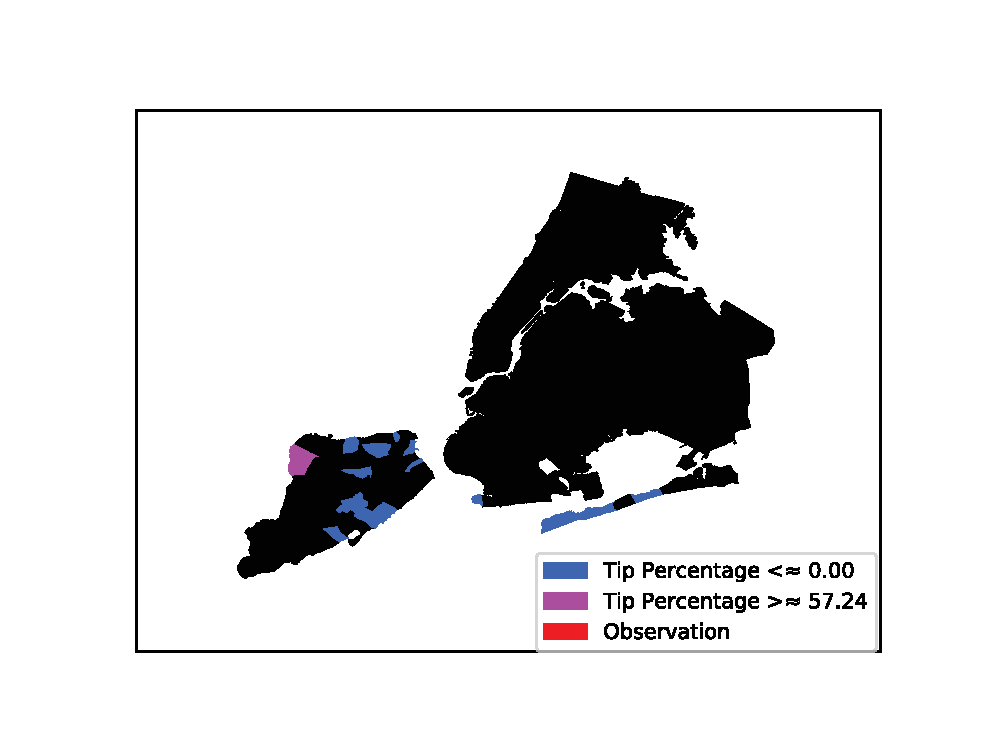
\includegraphics[width=\columnwidth]{spatial_explanation_example.eps}
\caption{An example of spatial explanation}
\label{fig:spatial_explanation_example}
\end{figure}

The polygons painted purple show polygons in the candidate explanation where the tip percentage is high, while polygons painted blue show candidate explanations where the tip percentage is low. It should be noted that $P$ has a high number of permutations. It is up to the approach to decide which polygons to include in the candidate explanation. For instance, hierarchical intervention may choose polygons in a spatial proximity while aggravation may choose otherwise.
\begin{figure}[ht]
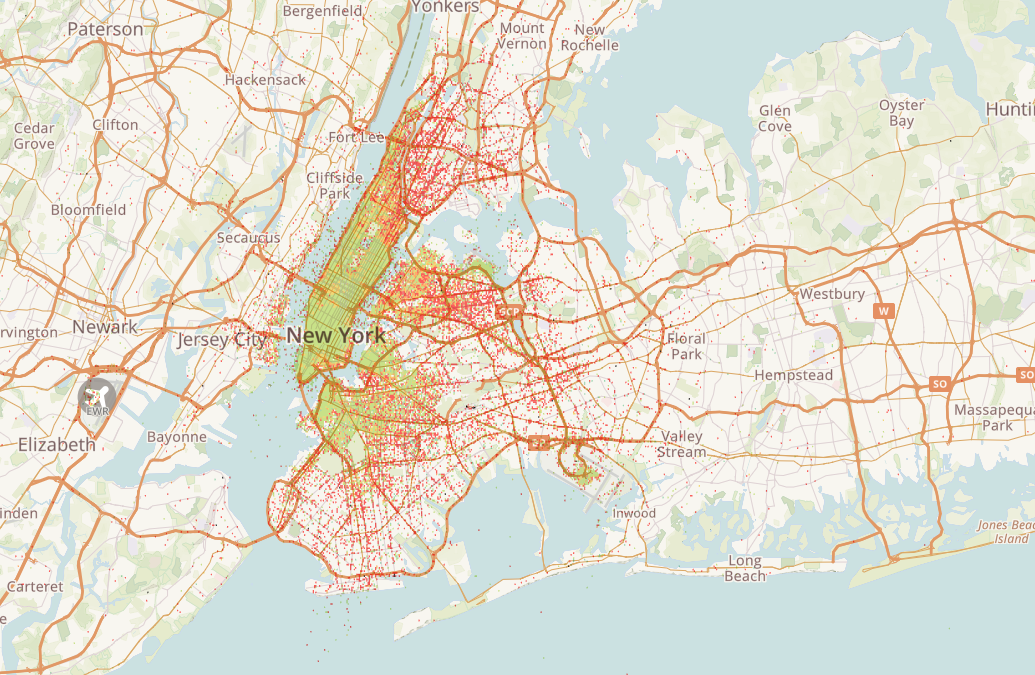
\includegraphics[width=\columnwidth]{scatter.png}
\caption{Heatmap for NYC trips for January 2016}
\label{fig:square_unit_grid}
\end{figure}

Another interesting consideration when we are talking about spatial explanations is the density of the data. Fig.~\ref{fig:square_unit_grid} shows the heatmap for tip percentage with respect to pickup coordinates. It is interesting to observe that the explanations provided in Fig.~\ref{fig:spatial_explanation_example} are all areas with low density of data. One of the reasons for this is because each approach takes some liberty with our definition of the taxonomy. Even though, we defined $P$ to contain all permutations of polygons, an approach may use limited polygons, such as neighborhoods or zones. The way the explanation is ranked also plays a large role.

\subsection{Spatial explanations for spatial observations}
\label{sec:spatial_spatial}
In the last two classes of our taxonomy, we only looked at non spatial observations. In this class however, we will look at spatial observations. Spatial observations are similar to non spatial observation. Both spatial and non spatial observations are represented by an aggregate query. The difference is that spatial observations have a polygon in the predicate. The spatial explanation in this class can be defined in the same way as in Section~\ref{sec:spatial_nonspatial}.

\begin{wrapfigure}{R}{0.5\textwidth}
  \begin{center}
    \includegraphics[width=0.48\textwidth]{spatial_spatial_vertical.eps}
  \end{center}
  \caption{An example of spatial explanation for a spatial observation}
\label{fig:spatial_spatial_vertical}
\end{wrapfigure}



Fig.~\ref{fig:spatial_spatial_vertical} shows an example of a spatial explanation for a spatial observation. The observation, in this case, is the average tip percentage when the pickup zone is LaGuardia airport. The candidate explanation displayed are also based on tip percentage, though they could have been any other attribute as well. Introducing a spatial predicate has a large observable impact on the explanation compared to the one in Section~\ref{sec:spatial_nonspatial}

There is a visible difference between the explanations in Fig.~\ref{fig:spatial_explanation_example} and Fig.~\ref{fig:spatial_spatial_vertical}. This is because Fig.~\ref{fig:spatial_explanation_example} shows the explanation for average tip percentage in general where the entire New York area is covered in the observation. Fig.~\ref{fig:spatial_explanation_example} on the other hand shows the explanation in the context of the dropoff zone for the trip where the pickup zone is LaGuardia airport.


\section{Studied Approaches}
\label{sec:approaches}
There are three main approaches that we use in this thesis. Aggravation, Intervention and Salient Features. We also introduce hierarchical intervention. This approach is an extension of intervention which takes spatial clusters into account. Originally, Aggravation and Intervention were used in a non spatial context in related works\citep{chirigati2016data}. However, we extended these solutions to fit into our spatial taxonomy.

\subsection{Aggravation}
\label{sec:aggravation}

The first approach we will look at for explanation is aggravation. This approach tries to look at tuples which 'aggravate' the results. The main idea is to calculate the value of the observation for each candidate explanation. The candidate explanation with the highest value has the highest weight as the explanation.

Let $q$ be our observation query(aggregate query). Let $\phi$ be our candidate explanation. Let $D_\phi$ be the dataset that satisfies our candidate explanation i.e. $D_\phi = \sigma_\phi(D)$. Let $Q$ be a scalar function that takes in a dataset and gives the value obtained when $q$ is applied to this data. The degree of candidate explanation, $\delta_{agg}$, by aggravation can be simplified as $Q(D_\phi)$.

In order to have a degree of explanation which is high when we are closer to our desired explanation, we need to have a direction for our explanation. For example, if we want to observe high values of tip percentage in the NYC TLC data, our direction will be high. If we want to observe lower values of tip percentage, our direction will be low. If our direction is low, we are interested in the lower values. However, since we want our degree of candidate explanation to be higher when we have the desired candidate explanation, we can simply reassign its value.

\begin{equation}
\delta_{agg}:=
    \begin{cases}
      Q(D_\phi), & \text{if}\ direction=high \\
      -Q(\phi), & \text{otherwise}
    \end{cases}
\end{equation}

% Bucketing values
In order to decrease the number of permutations for candidate explanations, we can bucket the values. Consider an attribute $a$ in the dataset. Let $V_a$ represent each value that $a$ can takes up, where $V_a=\{v_1,v_2,...,v_n\}$ and $n$ is the number of tuples. Let the minimum value in $V_a$ be represented by $a_{min}$.The mean value, $\mu$, is defined as $\frac{\Sigma_iv_i}{n}$. The standard deviation, $\sigma$, is defined as $\sqrt{\frac{1}{n-1}\Sigma_i(v_i-\mu)^2}$. Each value is assigned to a bucket. Let $b_i$ be the bucket the value, $v_i$ is assigned to. Then $$b_i = \bigg \lfloor\frac{v_i-a_{min}}{\sigma} \bigg \rfloor$$

Now, instead of using all the permutations in $V_a$ as part of our candidate explanations, we can rather use all the distinct values of buckets. The predicate represented by each bucket $b_i$ is simply
$$ a \geq (a_{min}+b_i\times\sigma) \wedge a < (a_{min}+b_i\times(\sigma+1))$$
This decreases the number of permutions for candidate explanations by a factor of $\frac{1}{\sigma}$. As a hands on example of this approach consider the observation on the NYC TLC data represented in Query~\ref{qry:aggregate}.

\renewcommand{\lstlistingname}{Query}% Listing -> Algorithm
\begin{lstlisting}[language=SQL, caption=Aggregate Query for average tip percentage, label=qry:aggregate]
SELECT AVG(trip_distance) FROM
FROM nyc_data
\end{lstlisting}

We are interested in the candidate explanation in the context of the number of passengers. The top explanation for this observation gives $Q=6.00$, $b_i=3$. Since we know the bucket and $\sigma$. The explanation predicate turns out to be $passenger\_count \geq 3.97 \wedge passenger\_count < 5.30$. If you are a yellow cab driver, this explanation may tell you to be prepared for a long trip if you have four or five passengers.

Now that we have described the aggravation approach for the nonspatial case, we can extend it to handle spatial observations and explanations. We introduce a dataset of polygons $P$. The set $P$ consists of distinct non overlapping polygons over our dataset $D$. Let $s$,$t$ be the spatial attributes in $D$. Each tuple in $P$ has two attributes: $polygon\_id$, and $polygon$. We create a new dataset
$$D' \leftarrow D \bowtie_{contains(P.polygon,(s,t))} P$$

Now we can use our spatial candidate explanations and observations defined in our taxonomy(Section~\ref{sec:taxonomy}) on out new dataset $D'$

Fig.~\ref{fig:spatial_spatial_vertical} can be considered as an example of spatial aggravation where the spatial partitioning is based on taxi zones as dropoff locations. The observation is the tip percentage where the pickup zone is LaGuardia airport.

\subsection{Intervention}
\label{sec:intervention}

Intervention is an approach inspired by the concept of influence. It builds on the aggravation approach(Section~\ref{sec:aggravation}). Intervention tries to measure how much our observations would change had our explanation not been present. Let $D$ be the dataset we are interested in. Let $Q$ be a function which returns the value of our observation given a dataset. Keeping our taxonomy in context, this means $Q$ returns the value of our aggregate observation query. Let $\phi$ be our candidate explanation. Let $\Delta_\phi \leftarrow \sigma_\phi(D)$. Let $D_\phi = D - \Delta_\phi$. The direction of our observation can either be \textit{high} or \textit{low} depending on whether we are interested in the greatest or least values of observation respectively. Our degree of candidate explanation by intervention, $\delta_{int}$, can then be expressed as,
\begin{equation}
\delta_{int}:=
    \begin{cases}
        -Q(D_\phi), & \text{if}\ direction=high \\
        Q(D_\phi), & \text{otherwise}
    \end{cases}
\end{equation}

We want the degree of candidate explanation by intervention to be higher the closer we are to the direction of the observation, therefore, we use the negative value when the direction is high. If the influence of the candidate explanation is high, it will result in a low observation value once the candidate explanation is removed from the dataset.

Since intervention extends the idea presented by aggravation, it has similar issues when it comes to the number of permutations for candidate explanations. Similar to our approach in aggravation(Section~\ref{sec:aggravation}), we can reduce the number of permutations by bucketing the attributes. We can extend intervention for spatial observations and explanations the same way we did for aggravation. The set $P$ consists of distinct non overlapping polygons in our dataset $D$. Let $s$,$t$ be the spatial attributes in $D$. Each tuple in $P$ has two attributes: $polygon\_id$, and $polygon$. We create a new dataset
$D' \leftarrow D \bowtie_{contains(P.polygon,(s,t))} P$. Spatial observations can now be defined as aggregate queries with a predicate containing $P.polygon$. Candidate spatial explanations can be defined as candidate explanations containing $P.polygon$ as emphasized in our taxonomy(Section~\ref{sec:taxonomy}).

\begin{figure}[ht]
\begin{center}
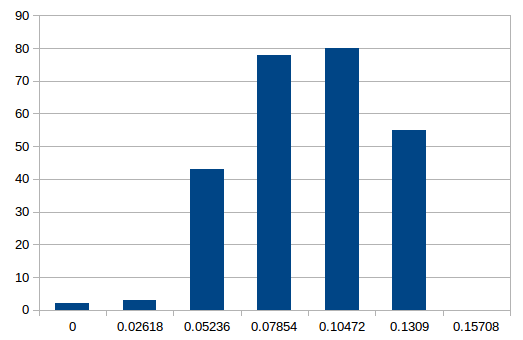
\includegraphics[width=0.5\columnwidth]{spatial_aggravation_histogram.png}
\end{center}
\caption{Number of Zones against Degree of Spatial Aggravation}
\label{fig:spatial_aggravation_histogram}
\end{figure}

\begin{figure}[ht]
\begin{center}
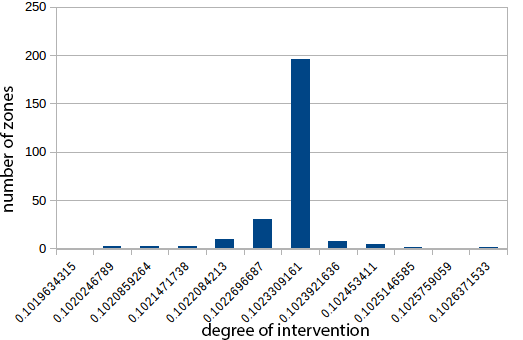
\includegraphics[width=0.5\columnwidth]{spatial_intervention_histogram.png}
\end{center}
\caption{Number of zones against their degree of Spatial Intervention}
\label{fig:spatial_intervention_histogram}
\end{figure}

In order to compare the differences between aggravation and intervention, it is helpful to look at their degrees of aggravation and intervention respectively. As an example, we look at the NYC TLC data where $P$ is the set of taxi zones. Fig.~\ref{fig:spatial_aggravation_histogram} shows a histogram for the number of taxi zones which fall inside different range of the degree of candidate explanation by aggravation. Fig.~\ref{fig:spatial_intervention_histogram} shows a similar histogram for the number of zones between certain ranges for the degree of candidate explanation by intervention. The observation in both cases is the average tip percentage. The degrees of explanation and the number of zones represent the domain and range, respectively. It is immediately evident from these two histograms that the domain for explanation by aggravation is 150 times larger than intervention while the range for explanation by intervention is 2.5 times larger than aggravation in this instance of the problem. The reason for having a small domain for intervention is because the influence of removing one of the zones on the observation is very small, whereas, each zone may have a large difference in average tip percentage compared to other zones. We will look further into the implications of these differences when we evaluate these approaches(Section~\ref{sec:evaluation}).

\subsection{Salient Features}
\label{sec:salient_features}

Another approach for finding explanations is the use of salient features. As the name suggests, salient features intend to highlight portions of data which stand out. One of the examples which illustrates this can be seen in Fig.~\ref{fig:yellowstats}. The figure shows the average number of taxi trips per day over the course of a month. There is a large noticeable decline in the number of trips. The data representing this decline can be considered as a salient feature. Salient features like these tell a lot about the data. For example, if you were to look up the date illustrated in the example where the number of taxi trips drops, you would find that there was a travel ban because of extreme weather conditions.

Salient features are based on temporal or spatio temporal scalar functions. This approach does not work with non-temporal functions. We define two types of scalar functions: 1-D scalar functions and 2-D scalar functions. 1-D scalar functions map time to a scalar value. For example, the data presented in Fig.~\ref{fig:yellowstats} maps time to the number of taxi trips. 2-D scalar functions map time and space to a scalar value.  Fig.~\ref{fig:spatial_explanation_example} shows an example of a 2-D scalar function for one time step. Since our taxonomy is concerned with only the spatial domain of this problem, we will be considering a 2-D scalar function where one time step covers the entire scope of our dataset, i.e. 1-D scalar function based on space. We go from 2-D to 1-D by only considering the entire time range as a single entity. It might be easier to understand this by considering a rectangle and a line. If a rectangle only has a unit width, it forms a line.

Now that we understand what salient features are, the natural question would be how to find salient features in a dataset. In order to calculate salient features, we define two threshold values $\theta^+$ and $\theta^-$. \textit{Positive salient features} are the parts of our scalar function where its value is greater than $\theta^+$ i.e. $f^{-1}([\theta^+, \infty))$. \textit{Negative salient features} are the parts of our scalar function where its value is less than $\theta^-$ i.e. $f^{-1}((-\infty, \theta^-])$. The local maxima and minima are referred to as \textit{critical points} i.e. $\nabla f = 0$

Our extension of this approach for spatial explanation stems from the fact that each feature can be represented as a predicate. For instance if we consider the function represented in Fig.~\ref{fig:yellowstats}. Let $\theta^-$ be 20,000. Then the negative salient feature can be represented as a predicate based on time and the number of trips. In the case of a 2-D scalar function, the predicate would be based on the time, attribute, and a polygon. In case of a 1-D spatial scalar function, the predicate would consist of a polygon, and an attribute. In order to calculate an explanation, we measure the co-relation between scalar functions of different attributes in a dataset. Let $f_1$ be the scalar function for one attribute and $f_2$ be the scalar function of another attribute. Let $F_1$ and $F_2$ be the features of $f_1$ and $f_2$ respectively. We define $F$ to be the set of features both $f_1$ and $f_2$ have in common, where  $ F = F_1 \cap F_2$. $f_1$ and $f_2$ are \textit{feature related} at a point $x$ if $x \in F$. $f_1$ and $f_2$ can be positively or negatively related. Let $F^+ = F_1^+ \cap F_2^+$ where $F_1^+$ and $F_2^+$ are positive features of $f_1$ and $f_2$ respectively. Let $F^- = F_1^- \cap F_2^-$ where $F_1^-$ and $F_2^-$ are negative features of $f_1$ and $f_2$ respectively. Then $f_1$ and $f_2$ are positively related at $x$ if $x \in F^+$  or $x \in F^-$. $f_1$ and $f_2$ are negatively related at $x$ if $x \notin F^+\ \text{and}\ x \notin F^-\ \text{and}\ x\in F$.

The value of relationship score, $\tau$, can help us decide whether two attributes are co-related. If the attributes are related, then their features can be represented as candidate explanations. Let $p$ be the set of positive relations in $F$. Let $n$ be the set of negative relations in $F$. Then,
$\tau = \frac{|p|-|n|}{|F|}$


Our system builds on the implementation of the salient features by \cite{chirigati2016data} in their work on the Data Polygamy framework. Calculating salient features consists of three main steps: Pre processing, aggregation, and indexing. Each step in this process is implemented as a map reduce operation.

In the preprocessing step, the spatial and temporal attributes of the dataset are used to select the data. The spatial and temporal attributes form the key in the MapReduce job while the average of our attributes forms the value. In the aggregation step, the scalar functions are generated for the data. Each attribute in our dataset is represented by a different scalar function. Several scalar functions are calculated for each attribute for each spatio temporal resolution e.g. the spatio temporal resolution of 'hour' and 'neighborhood' has a different scalar function compared to that for 'day' and 'ZIP code'. The next step consists of indexing the data. Indexing consists of creating a graph out of the aggregated data. Each node in the graph represents a point in the spatiotemporal domain. It may be convenient to think of this as a 3-D graph where two axes represents space and another represents time. A node is connected to another node if they are adjacent to each other in space(e.g. two neighborhoods next to each other) and time. The value of each node is the average attribute value. Due to the nature of the data, some points in the graph might be missing. The indexing step linearly interpolates the missing points in the graph. The 2-D scalar functions we calculated are finally used to calculate whether each node in our graph is a negative salient feature or positive salient feature.

After the salient features are calculated we need to measure how well they explain the data. We do this by finding the relationship score between the observation scalar function and the scalar function for the remaining attributes in our dataset. The non spatial explanation consists of our threshold values while the spatial explanation consists of the polygons represented by the co-related salient features.

\chapter{Spatial Explanations using Hierarchical Intervention}
\label{chp:proposed}
\label{sec:hei_intervention}

\section{Introduction}
Hierarchical Intervention is an extension of the intervention approach. The idea behind hierarchical intervention is to improve our explanations by grouping together spatially colocated polygons in our candidate explanation. We divide the space into a set of levels. The first level contains the entire space as one cluster, while the last level contains each zone or each point in each cluster.

\section{Spatial Partitioning/Clustering}
There are several approaches to cluster data. Each clustering approach has a large impact on the resulting explanations. In order to understand the issues with explanations using spatial clustering, we need to have an understanding of the clustering approaches.

\subsection{R-Tree}
An R-Tree is a data structure which is commonly used for spatial data indexing. The idea behind the R-Tree is similar to the idea behind a binary tree i.e. It is faster to query data if it is stored in the form of a hierarchy\citep{guttman1984r}. In an R Tree this hierarchy exists in the form of Minimum Bounding Rectangles(MBR).

\begin{figure}[ht]
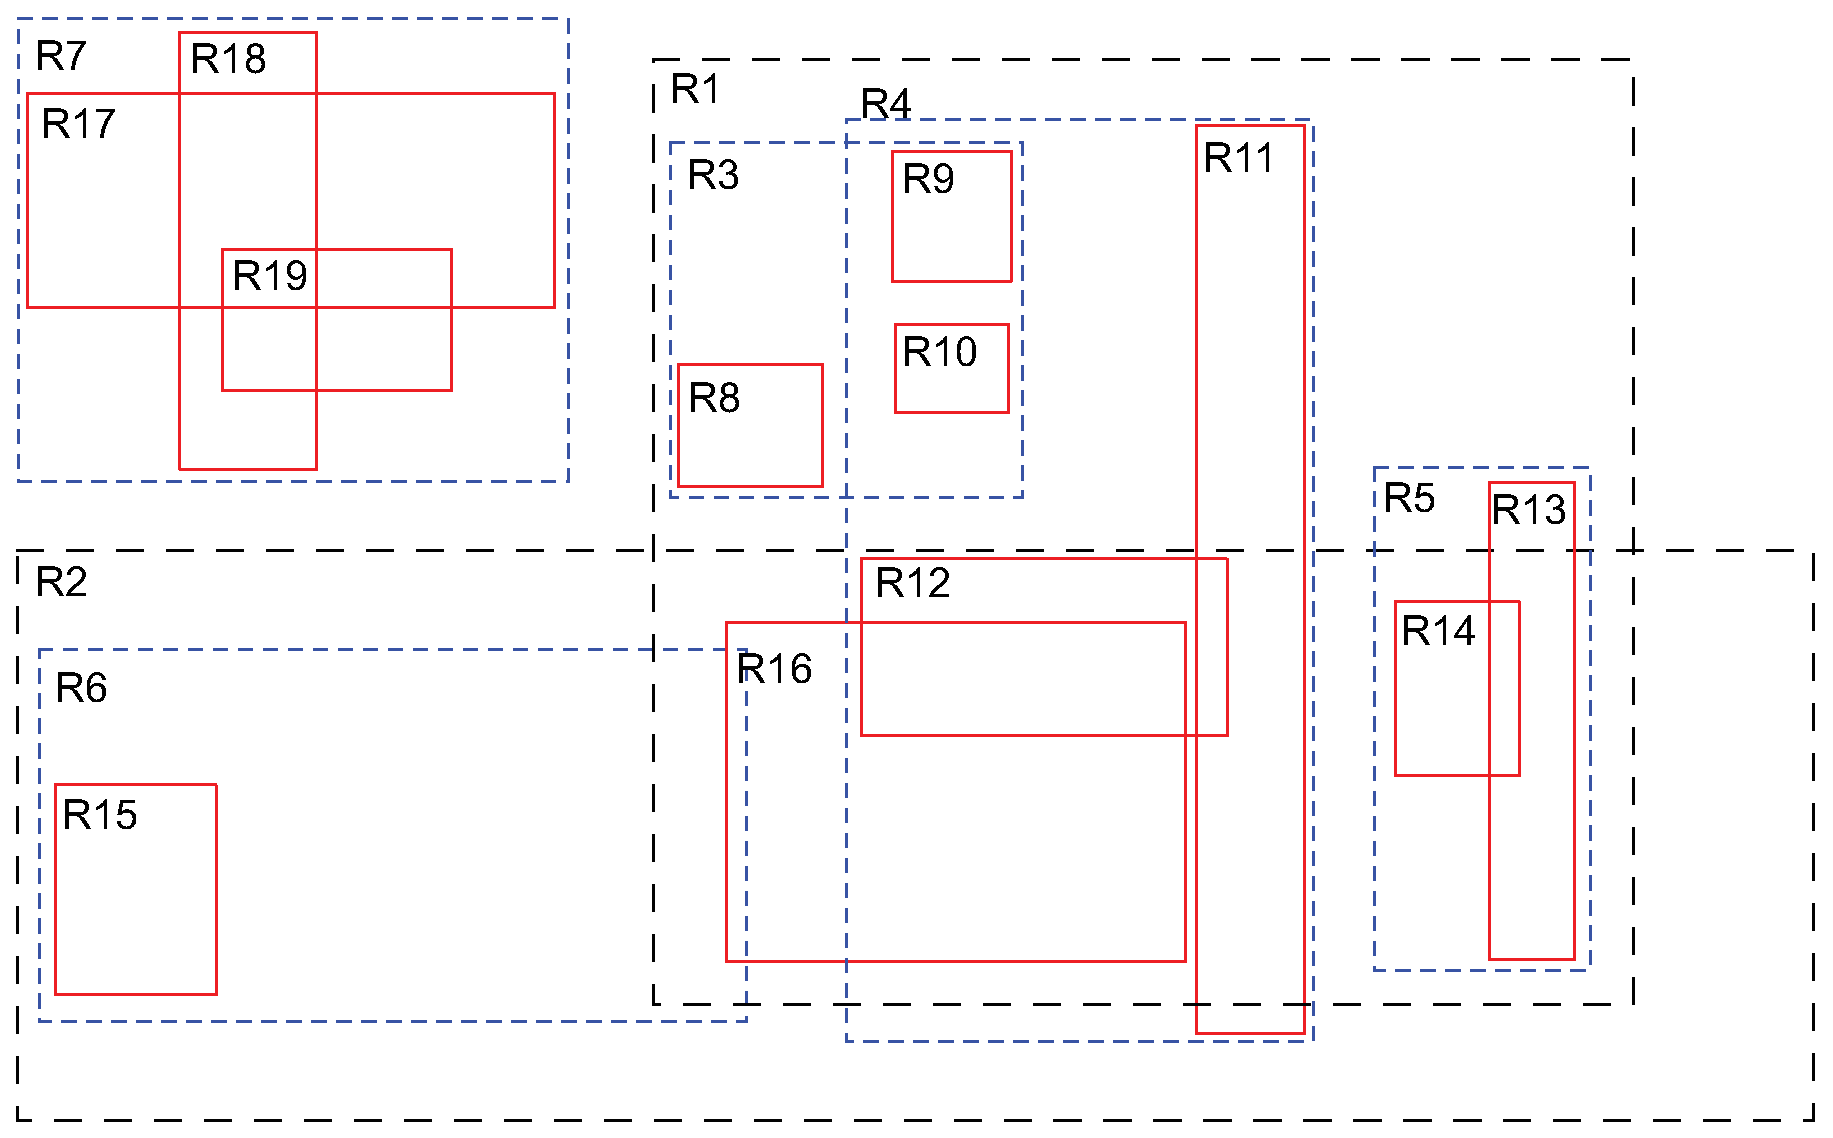
\includegraphics[width=\columnwidth]{rtree}
\caption{An illustration of R-Tree}
\label{fig:rtree}
\end{figure}

The top level of an R Tree consists of a set of MBRs which cover a large spatial area. Each MBR can now be subdivided into further MBRs which makes up the second level of the tree and so forth. At the leaf nodes of the tree, each node consists of a single object in our underlying data.

There are three main considerations when building an R Tree: insertion, deletion, and search. In order to insert data, it is important to consider that the tree is balanced. A balanced tree results in faster search since the depth of the tree is reduced. The same thing needs to be taken into consideration with deletion.
In order to insert an element, a heuristic is usually involved. The main objective when inserting into an R-Tree is to minimize the splitting and enlargement. If an element can be inserted into an existing MBR, then it is preferred. Otherwise, existing MBR's are either split or enlarged.

When elements from an R-Tree are deleted, the parent nodes are also taken into consideration. This is because deleting elements may result in a change in the parent MBR as well unlike a B-Tree. An R-Tree maintains a minimum utilization constant into consideration when deleting. If a node in the R-Tree is below the minimum utilization, the elements are reinserted.

Finally the main purpose of constructing an R-Tree is to optimize search speed. If the branching factor of the R-Tree is $\lambda$ and there are $n$ elements that are indexed, then the search cost of the R-Tree is $\log_{\lambda}{n}$ assuming that the tree is balanced.


\subsection{R*-Tree}
R* Tree is a variation of R-Tree\citep{beckmann1990r}. The objective of an R*-Tree is to minimize overlaps and coverage in an R-Tree. It also optimizes for margin and area. The idea behind R*-Tree which helps in achieving its objective is to use the perimeter of the MBR as a heuristic when splitting and creating R-Trees.

Unlike R-Trees the insert operation of an R* Tree also incorporates deletion. When an element is added to an R-Tree, an existing MBR is either extended or split. However, ordering of the insertion in an R-Tree deforms existing MBRs and may lead to more coverage. R* Tree solves this problem by removing elements from nodes and reinserting them. Splitting of MBRs is also based on perimeter. There are multiple ways to split an MBR but if its split based on least resulting perimeter as a heuristic, it leads to better partitioning which leads to less overlaps.

The search and delete operations of an R* Tree are the same as an R Tree.

\subsection{K-means clustering/Voronoi partitioning}
K means clustering is an algorithm designed to cluster a group of points. As the name suggests, the user decides the number of clusters that he/she wants. $K$ represents the number of clusters. The algorithm randomly selects $k$ seed points. The seed points can also be selected using a heuristic to improve the clustering. The points closest to each of the seed points form clusters. The k means algorithm is iterative. Which means it doesn't end there. The centroids of the clusters are used as new seed points and the process is repeated until the centroids are constant. Algorithm~\ref{alg:kmeans} shows our version of the kmeans algorithm where the selectivity is used as a metric for judging the clusters.

% TODO Add reference to greedy hierarchical clustering
% Let $D$ be our spatial dataset. Let $P$ be a set of distinct polygons over our dataset $D$. We define a set of distinct clusters of polygons $P_h$. The polygons can be clustered in many different ways but we used greedy hierarchical clustering because of its speed and relevance to the problem. Let $C$ be the set of centroids in $P$ i.e. $\forall p_i \in P$, $c_i$ is the centroid for $p_i$, where $c_i \in C$. We define a set of $n$ levels, $L = \{l_1, l_2,...,l_n\}$. We represent each centroid in $C$ on a cartesian plane where $x_i$ is the first dimension of the centroid $c_i$ and $y_i$ is the second dimension of the centroid $c_i$. Let $x_{min}$, $x_{max}$ be the minimum and maximum value for $x_i$ respectively. Let $y_{min}$, $y_{max}$ be the minimum and maximum values of $y_i$ respectively. There is a radius associated with each level in $L$. Let $r_i$ be the radius for level $l_i$ in $L$, We can define $r_i$ in general as,
% $$r_i = \frac{\sqrt{(y_{max}-y_{min})^2+(x_{max}-x_{min})^2}}{2^{i-1}}$$

% The set of clusters,$G_i$, for level $l_i$ can be defined as $G_i=\{p_k|(x_k^2 + y_k^2 < r_i^2)\}\forall p_k \in P$. Any possible set cover of $P$ in $G_i$ can now be considered for inclusion in $P_h$. One implementation of this approach is covered in Section~\ref{sec:hie_impl}


\subsection{Hierarchical Greedy Clustering}
Hierarchical Greedy Clustering is a popular algorithm in data visualizations because of its speed. The idea behind this algorithm is to randomly select points and create clusters around them.

Let $D$ be our spatial dataset. Let $P$ be a set of distinct polygons over our dataset $D$. We define a set of distinct clusters of polygons $P_h$. Let $C$ be the set of centroids in $P$ i.e. $\forall p_i \in P$, $c_i$ is the centroid for $p_i$, where $c_i \in C$. We define a set of $n$ levels, $L = \{l_1, l_2,...,l_n\}$. We represent each centroid in $C$ on a Cartesian plane where $x_i$ is the first dimension of the centroid $c_i$ and $y_i$ is the second dimension of the centroid $c_i$. Let $x_{min}$, $x_{max}$ be the minimum and maximum value for $x_i$ respectively. Let $y_{min}$, $y_{max}$ be the minimum and maximum values of $y_i$ respectively. There is a radius associated with each level in $L$. Let $r_i$ be the radius for level $l_i$ in $L$, We can define $r_i$ in general as,
$$r_i = \frac{\sqrt{(y_{max}-y_{min})^2+(x_{max}-x_{min})^2}}{2^{i-1}}$$

The set of clusters,$G_i$, for level $l_i$ can be defined as $G_i=\{p_k|(x_k^2 + y_k^2 < r_i^2)\}\forall p_k \in P$. The algorithm for the implementation of this approach is covered in Section~\ref{sec:hie_impl}.

Greedy Hierarchical Clustering turned out to have a drawback when we use it for explanations. It selects seed points randomly. This means that in each level, the clusters can be highly imbalanced. We compared this approach to K means(Voronoi partitioning)\citep{hartigan1979algorithm,aurenhammer2000voronoi}, R Tree\citep{guttman1984r} and R* Tree\citep{beckmann1990r}.

The main idea behind the hierarchical intervention approach, regardless of the partitioning algorithm, is to help us in increasing the domain for our degree of explanation. Since, intervention is a subset of this approach the domain is at least as large as that for intervention.


\section{Extending Hierarchical Intervention}
\label{sec:extending_hi}

In order to get the most out of Hierarchical Intervention, we introduce two new metrics: Intensity and Influence.

\subsection{Intensity}
\label{sec:intensity}

%What is relevance
We define intensity as a metric which measures the standalone value of the explanation. The relevance metric borrows a lot from our definition of aggravation. It might be convenient to think of a web search engine when we are looking at the intensity metric. When we use a search engine, we provide a search term as a query. The search engine looks at all the pages in its database and returns the results in order of relevance. The top results in the search engine may not have a significant effect on the entire web if they were to be removed. However, the top result in the search engine has the highest relation to the data. For example, the top result for a search engine which uses tf-idf might be a page containing the highest frequency of the search term\citep{robertson2004understanding}.

%Formal definition of relevance
Let $D$ be our dataset. Let $\phi$ be our candidate explanation. Let $R$ be the function which maps our dataset to the value of our observation. Then we can define intensity as,
$$intensity = |R(\sigma (D)) - R(\sigma_\phi (D))|$$

\subsection{Influence}
\label{sec:influence}
% What is influence
We define influence as a metric which measures the value of the explanation compared to the entire dataset. The influence metric borrows from our definition of intervention. The influence metric measures how much the observation would be affected if we remove the data related to our explanation(the \textit{influence} of our explanation on the observation). We can use the analogy of the search engine again here. One of the earliest algorithms used by Google to rank webpages used links to other pages\citep{brin1998anatomy}. The page which was linked the most on a variety of websites was ranked higher. If you remove a highly relevant page, many other pages might not exist. Influence uses the same principle.

%Formal definition of influence
Let $D$ be our dataset. Let $\phi$ be our candidate explanation. Let $R$ be the function which maps our dataset to the value of our observation. Then we can define relevance as,
$$influence = |R(\sigma(D)) - R(\sigma_{\neg \phi} (D)) |$$

The greater the value of influence, the more its impact on the observation.

Our evaluation metrics suggest that influence and intensity explain data in different ways. Explanations with higher influence tend to give predicates which cover a larger area while explanations with higher intensity tend to give predicates which cover a small area. We can balance out these two metrics according to the preferences of the observer. We define the \textit{explanation index}, $\epsilon$ as:
$$\epsilon = \alpha \times influence + (1-\alpha) \times intensity$$
$\alpha$ is the \textit{explanation coefficient}. It is a variable whose value is decided by the user.

Explanations given by Hierarchical Intervention can be ranked on the basis of the explanation index.


\section{Implementation}
\label{sec:implementation}
We created an implementation of the our system as a proof of concept. Our system uses a web based GUI for the visualizations while the backend processing is done using Spark\citep{shanahan2015large}. We borrowed from the MapReduce implementation of Salient Features from the Data Polygamy Framework\citep{chirigati2016data}. There are three main stages in our system pipeline: Preprocessing, User Input and Explanation Visualization. The preprocessing stage is different for each approach to explanation. The user input stage can be divided into two further parts: The user observation, and the type of explanation the user is interested in. An example of the explanation approach would be intervention. The user observation can be one of the attributes the user wants to observe e.g. a mathematical expression spanning several aggregate queries.


\label{aggravation_impl}
The aggravation approach that we use makes several optimizations to the naive approach one may come up with. A naive approach may consider each candidate explanation and calculate the degree of explanation by aggravation for each one. However, using such an approach would take a long time. If the attribute which we are looking into for explanation has $m$ possible values, it would take $O(m)$ queries to come up with top explanations. If we have $r$ rows in our dataset and each observation query has a linear time complexity, our total time complexity would be $O(rm)$. We can reduce the time complexity by a large factor if we make each candidate explanation cover a larger range of the dataset.

%Talk about bucketing
As mentioned in Section~\ref{sec:aggravation}, we use bucketing to reduce the number of permutations. We use the standard deviation, $\sigma$, of each attribute to separate values which are near the average from the others. We can get the minimum and standard deviation of each attribute over a single iteration of our table in $O(r)$ time. Since the bucket for each value of the attribute can be calculated in constant time, we create a new table containing the bucket value of the attribute in $O(r)$ time.

%Talk about grouping
Since we bucketed our data, the number of candidate explanations have been reduced to $O(\big(\frac{m}{\sigma}\big))$. However, there is still room for improvement. Our observation is always an aggregate query. If we group on the explanation attributes, we can still get all of the corresponding values of the observation in one iteration of the data, making our time complexity $O(r)$.

%Talk about zoning
Another component of our system is spatial data. Our system is designed to handle spatial observations and explanations. When given a spatial observation, our system filters out the data with the spatial predicate given in the observation. The remaining data is used just like any other explanation task. Spatial Explanations, on the other hand, require a bit more work. Given a set of polygons, doing a spatial join with the data is a very expensive process. Our system performs a spatial join once and assigns each tuple an ID based on which polygon it belongs to. The ID can now be used like a regular attribute for explanation.


\label{intervention_impl}

%Talk about grouping
Intervention is another approach that our system uses. Some of the work we did to optimize aggravation cannot be used to improve the time complexity for intervention. This is because intervention looks at the effect of removing data. While we could use a single iteration of the data for aggravation. We cannot do so for intervention because removing one portion of the data completely changes what the observation looks like. We can still use bucketing to reduce the number of combinations.


\subsection{Hierarchical Intervention}
\label{sec:hie_impl}
Hierarchical intervention is an improvement on top of the intervention approach. The main idea behind hierarchical intervention is to group spatially colocated points/polygons together in an attempt to improve explanations. We use a partitioning algorithm to create clusters. The base case of our algorithm consists of clusters with a single node each. This makes the results of intervention a subset of the results of hierarchical clustering. Algorithm~\ref{alg:hie} highlights the algorithm that we used for our implementation of greedy hierarchical clustering. Note that each level in the hierarchy is a set cover of all the nodes.

Greedy Hierarchical Clustering is an iterative algorithm. The base case(Algorithm.~\ref{alg:hie};27) is when we reach the lowest level in the hierarchy where we have individual points or zones. We start off with the highest level in the hierarchy(Algorithm.~\ref{alg:hie};4). We select random points and form clusters around them(Algorithm.~\ref{alg:hie};16). In the following iteration we reduce the size of the cluster by a constant factor(Algorithm.~\ref{alg:hie};8) and repeat until we reach the base case.


% Talk about clustering
\begin{algorithm}
\caption{Algorithm for Hierarchical clustering}\label{alg:hie}
\begin{algorithmic}[1]
\Procedure{Cluster}{$max\_radius,points$}
  	\State $input: max\_radius, points$
      \State $output: hierarchy\_of\_clusters$
   	\State $level \gets 0$

  	\State $isBaseCase \gets false$
  	\While{isBaseCase = false}
  	    \State $level \gets level + 1$
  	    \State $levelRadius \gets \frac{max\_radius}{2.0^{level}}$

  	 	\State $hierarchy \gets \emptyset$

  	    \State $unusedPoints \gets \emptyset$

      	\For{$point \gets points$}
      		\State $unusedPoints \gets unusedPoint \cup point$
      	\EndFor

      	\While{$unusedPoints.size > 0$}
  			\State $cluster \gets \emptyset$

  			\State {$centroid \gets $random point from points}

  			\For{$point \gets unusedPoints$}
  				\If{point inside levelRadius}
  					\State $cluster \gets cluster \cup point$
  					\State $unusedPoint \gets unusedPoints - point$
                 \EndIf
  			\EndFor

  			\State $hierarchy \gets hierarchy \cup cluster$

      	\EndWhile
        \algstore{myalg}
    \end{algorithmic}
    \end{algorithm}
    \begin{algorithm}
    \begin{algorithmic} [1]
    \algrestore{myalg}
      	\State $hierarchy\_of\_clusters \gets hierarchy\_of\_clusters \cup \{level,hierarchy\}$

      	\State $isBaseCase \gets true$

  		\For{$cluster \gets heirarchy$}
  			\If {$cluster.size > 1$}
  				\State $isBaseCase \gets false$
  			\EndIf
  		\EndFor
  	\EndWhile
  	\State \textbf{return} $hierarchy\_of\_clusters$

\EndProcedure
\end{algorithmic}
\end{algorithm}

\begin{figure}
%   \begin{algorithmic}[1]
%   % 	\State $input: max_radius, points$
%   %     \State $output: hierarchy_of_clusters$
%   %  	\State $level \gets 0$

%   % 	\State $isBaseCase \gets false$
%   % 	\While{isBaseCase = false}
%   % 	    \State $level \gets level + 1$
%   % 	    \State $levelRadius \gets \frac{max_radius}{2.0^{level}}$

%   % 	 	\State $hierarchy \gets \emptyset$

%   % 	    \State $unusedPoints \gets \emptyset$

%   %     	\For{$point \gets points$}
%   %     		\State $unusedPoints \gets unusedPoint \cup point$
%   %     	\EndFor

%   %     	\While{$unusedPoints.size > 0$}
%   %     		\State $numShapes \gets unusedPoints.size$
%   % 			\State $cluster \gets \emptyset$

%   % 			\State $centroid \gets random point from points$

%   % 			\For{$point \gets unusedPoints$}
%   % 				\If{$point inside levelRadius$}
%   % 					\State $cluster \gets cluster \cup point$
%   % 					\State $unusedPoint \gets unusedPoints - point$
%   % 			\EndFor

%   % 			\State $hierarchy \gets hierarchy \cup cluster$

%   %     	\EndWhile
%   %     	\State $hierarchy_of_clusters \gets hierarchy_of_clusters \cup \{level,hierarchy\}$

%   %     	\State $isBaseCase \gets true$

%   % 		\For{cluster \gets heirarchy}
%   % 			\If {cluster.size > 1}
%   % 				\State $isBaseCase \gets false$
%   % 			\EndIf
%   % 		\EndFor
%   % 	\EndWhile
%   % 	\State \textbf{return} $hierarchy_of_clusters$
%   \end{algorithmic}
\end{figure}

% \renewcommand{\lstlistingname}{Algorithm}% Listing -> Algorithm
% \begin{lstlisting}[language=JAVA, caption=Algorithm for Hierarchical clustering, label=alg:hie]
% int level = 0;
% // Base Case. Each cluster contains one shape
% boolean isBaseCase = false;
% while(!isBaseCase){
%     level += 1;
%     // radiusL0 contains all points (Hypotenuse of MBR)
%     Double levelRadius = radiusL0 / Math.pow(2.0, level);

%     // Initialize hierarchy
%     ArrayList<List<Integer>> heirarchy = new ArrayList<>();

%     // Initialize a list containing all the points that are not in any cluster
%     ArrayList<Integer> unusedPoints = new ArrayList<>();
%     for(Integer objectId: shapemap.keySet()){
%         unusedPoints.add(objectId);
%     }

%     // Add points to a cluster while they're unused
%     while(unusedPoints.size()>0){
%         int numShapes = unusedPoints.size();
%         ArrayList<Integer> cluster = new ArrayList<>();
%         // Randomly select a shape
%         int pivot =  (int) Math.floor(Math.random() * numShapes);

%         // Get all shapes in radius
%         Point centroid = shapemap.get(unusedPoints.get(pivot)).getCentroid();

%         Iterator<Integer> unusedIter = unusedPoints.iterator();
%         while(unusedIter.hasNext()){
%             Integer objectId = unusedIter.next();
%             Point shapeCenter = shapemap.get(objectId).getCentroid();
%             if(shapeCenter.distance(centroid)<levelRadius){
%                 cluster.add(objectId);
%                 unusedIter.remove();
%             }
%         }

%         heirarchy.add(cluster);
%     }

%     HeirarchicalCluster.put(level, heirarchy);

%     // Check if we reached the base case level
%     isBaseCase=true;
%     for(List<Integer> cluster: heirarchy){
%         if(cluster.size() > 1){
%             isBaseCase = false;
%             break;
%         }
%     }
% }
% \end{lstlisting}

While greedy hierarchical clustering helps in increasing the domain for the degree of explanation by intervention, the random selection of seed points makes the rate of change of influence and intensity(Section~\ref{sec:extending_hi}) over the levels of hierarchy very volatile. Our point is illustrated by fig.~\ref{fig:hieint_passenger_count}. The red line represents influence while the blue line represents intensity. One would expect the curves to be logarithmic. However, they more closely resemble a sinusoidal function.


In order to try to counter this problem, we used k means clustering. Algorithm~\ref{alg:kmeans} highlights our implementation of k-means clustering centered around our problem. The algorithm is designed to find the clusters based on a heuristic of giving more preference to balanced clusters i.e. each cluster has similar number of points.

\begin{algorithm}
\caption{Explanation Aware K means}\label{alg:kmeans}
\begin{algorithmic}[1]
\Procedure{Cluster}{$points, k, number\_of\_runs$}
    \State $cluster\_possibilities \gets \emptyset$
    \For{$i \gets 0, number\_of\_runs$}
      \State $cluster\_possibilities \gets cluster\_possibilities \cup ClusterOnce(points, k)$
      \State $i \gets i + 1$
    \EndFor

    \State $best\_clustering \gets \emptyset$
    \State $best\_distance \gets \infty$

    \For{$possibility \gets cluster\_possibilities$}
      \State $cluster \gets GetCluster(possibility, points)$
      \State $k\_distance \gets GetKMeansDistance(cluster)$
      \If{$k\_distance < best\_distance$}
        \State $best\_distance \gets k\_distance$
        \State $best\_clustering \gets cluster$
      \EndIf
    \EndFor

    \State \textbf{return} $best\_clustering$
\EndProcedure

\Procedure{GetKMeansDistance}{$clusters$}
    \State $max\_distance \gets -\infty$
    \State $min\_distance \gets \infty$

    \State {$centroids \gets$ centroids of $clusters$}
    \For{$centroid \gets centroids$}
      \State {$related\_cluster \gets$ cluster from centroid}
    \algstore{kmeansalg1}
    \end{algorithmic}
    \end{algorithm}
    \begin{algorithm}
    \begin{algorithmic} [1]
    \algrestore{kmeansalg1}
      \State $cluster\_weight \gets GetClusterWeight(related\_cluster)$
      \If{$cluster\_weight > max\_distance$}
        \State $max\_distance \gets cluster\_weight$
      \EndIf

      \If{$cluster\_weight < min\_distance$}
        \State $max\_distance \gets cluster\_weight$
      \EndIf
    \EndFor

    \State \textbf{return} $|max\_distance-min\_distance|$
\EndProcedure

\Procedure{GetClusterWeight}{$points$}
    \State $count \gets 0$
    \For{$point \gets points$}
      \State $count \gets count + 1$
    \EndFor
    \State \textbf{return} $count$
\EndProcedure

\Procedure{GetCluster}{$centroids, points$}
  \State $clusters \gets \emptyset$

  \For{$centroid \gets centroids$}
    \State $clusters \gets clusters \cup \{centroid, \{\}\}$
  \EndFor

  \For{$point \gets points$}
    \State $closest\_centroid \gets nil$
    \For{$centroid \gets centroids$}
    \algstore{kmeansalg2}
    \end{algorithmic}
    \end{algorithm}
    \begin{algorithm}
    \begin{algorithmic} [1]
    \algrestore{kmeansalg2}
      \If{$closest\_centroid = nil$}
        \State $closest\_centroid = centroid$
      \ElsIf{{distance from $centroid$ $<$ distance from $closest\_centroid$}}
        \State $closest\_centroid \gets centroid$
      \EndIf
    \EndFor
    \State {Add $point$ to cluster where the centroid is $closest\_centroid$}
  \EndFor

  \State \textbf{return} $clusters$
\EndProcedure

\Procedure{ClusterOnce}{$points, k$}
    \State $centroids \gets \emptyset$
    \State $selected\_points = \emptyset$
    \For{$i \gets 1, k$}
    \State {$random\_point \gets$} random point from $points$
    \While{$random\_point \in selected\_points$}
      \State {$random\_point \gets$} random point from $points$
    \EndWhile
    \State $selected\_points \gets selected\_points \cup random\_point$
    \State $centroids \gets centroids \cup random\_point$
    \State $i \gets i+1$
    \EndFor

    \While{true}
      \State $clusters \gets GetCluster(centroids, points)$
    \algstore{kmeansalg3}
    \end{algorithmic}
    \end{algorithm}
    \begin{algorithm}
    \begin{algorithmic} [1]
    \algrestore{kmeansalg3}
      \State $new\_centroids \gets \emptyset$
      \For{$centroid \gets centroids$}
        \State {$cluster \gets$ cluster for $centroid$}
        \State $sum\_x \gets 0$
        \State $sum\_y \gets 0$
        \State $num\_values \gets 0$
        \For{$point \gets cluster$}
          \State $sum\_x \gets sum\_x + point.x$
          \State $sum\_y \gets sum\_y + point.y$
          \State $num\_values \gets num\_values +1$
        \EndFor
        \State $avg\_point \gets (sum\_x/num\_values, sum\_y/num\_values)$
        \State $closest\_point \gets nil$

        \For{$point \gets cluster$}
          \If{$closest\_point = nil \vee$ distance of $point$ from $avg\_point$ $<$ distance from $closest\_point$}
            \State $closest\_point \gets point$
          \EndIf
        \EndFor

        \State $new\_centroids \gets new\_centroids \cup closest\_point$

      \EndFor

      \State $centroids\_same \gets true$
      \For{$new\_centroid \gets new\_centroids$}
        \State $centroid\_found \gets false$
        \For{$old\_centroid \gets centroids$}
    \algstore{kmeansalg4}
    \end{algorithmic}
    \end{algorithm}
    \begin{algorithm}
    \begin{algorithmic} [1]
    \algrestore{kmeansalg4}
          \If{$old\_centroid = new\_centroid$}
            \State $centroid\_found \gets true$
            \State \textbf{break}
          \EndIf
        \EndFor
        \If{$centroid\_found = false$}
          \State $centroid\_same = false$
          \State \textbf{break}
        \EndIf
      \EndFor
      \If{$centroids\_same$}
        \State \textbf{break}
      \Else
        \State $centroids \gets new\_centroids$
      \EndIf
    \EndWhile
    \State \textbf{return} $centroids$
\EndProcedure
\end{algorithmic}
\end{algorithm}

% \begin{lstlisting}[language=JAVA, caption=Algorithm for K means, label=alg:kmeans]
% public static HashMap<Point, List<PointDatum>> cluster(PointDatum[] pointData, int k, int numRuns){
%     // Generate Cluster Combinations
%     ArrayList<Point[]> clusterPossibilities = new ArrayList<>();
%     for(int i = 0; i<numRuns; i++){
%         clusterPossibilities.add(clusterOnce(pointData, k));
%     }

%     // Select the best combination
%     HashMap<Point, List<PointDatum>> bestClustering = null;
%     double bestDistance = Double.MAX_VALUE;
%     for(Point[] possibility: clusterPossibilities){
%         HashMap<Point, List<PointDatum>> tempCluster = getCluster(possibility, pointData);
%         double kdistance = getKMeansDistance(tempCluster);
%         if(kdistance<bestDistance){
%             bestDistance =kdistance;
%             bestClustering = tempCluster;
%         }
%     }

%     return bestClustering;
% }

% private static double getKMeansDistance(HashMap<Point, List<PointDatum>> clusters){
%     double max_distance = Double.MIN_VALUE;
%     double min_distance = Double.MAX_VALUE;

%     Set<Point> centroids = clusters.keySet();

%     for(Point centroid: centroids){
%         double clusterWeight = getClusterWeight(clusters.get(centroid));
%         if(clusterWeight>max_distance){
%             max_distance = clusterWeight;
%         }
%         if(clusterWeight<min_distance){
%             min_distance = clusterWeight;
%         }
%     }

%     return Math.abs(max_distance-min_distance);
% }


% private static double getClusterWeight(List<PointDatum> pointDatum){
%     double clusterWeight = pointDatum.stream()
%             .map(pd->{return pd.getValue();})
%             .reduce((value1,value2)->{return value1+value2;}).get();
%     return clusterWeight;
% }

% private static HashMap<Point, List<PointDatum>> getCluster(Point[] centroids, PointDatum[] pointData){
%     // Form clusters by assigning point to nearest centroid
%     HashMap<Point, List<PointDatum>> clusters = new HashMap<>();

%     for(Point centroid: centroids){
%         clusters.put(centroid, new ArrayList<>());
%     }

%     for(PointDatum pointDatum: pointData){
%         Point closestCentroid = null;
%         // Find closest centroid
%         for(Point centroid: centroids){
%             if(closestCentroid==null){
%                 closestCentroid = centroid;
%             }else if(centroid.distance(pointDatum.getPoint()) < closestCentroid.distance(pointDatum.getPoint())){
%                 closestCentroid = centroid;
%             }
%         }

%         clusters.get(closestCentroid).add(pointDatum);
%     }

%     return clusters;
% }

% static Point[] clusterOnce(PointDatum[] pointData, int k){
%     // Select centroids at random
%     ArrayList<Point> centroids = new ArrayList<>();

%     ArrayList<Integer> selectedIndices = new ArrayList<>();
%     for(int i=0; i<k; i++){
%         Integer randomIndex = (int)Math.floor(Math.random()*pointData.length);
%         while(selectedIndices.contains(randomIndex)){
%             randomIndex = (int)Math.floor(Math.random()*pointData.length);
%         }
%         selectedIndices.add(randomIndex);

%         centroids.add(pointData[randomIndex].getPoint());
%     }

%     GeometryFactory gf = new GeometryFactory();

%     // While True
%     while(true) {
%         // Get cluster
%         HashMap<Point, List<PointDatum>> clusters = getCluster(centroids.toArray(new Point[centroids.size()]), pointData);

%         // Update centroids
%         ArrayList<Point> newCentroids = new ArrayList<>();
%         for(Point centroid: centroids){
%             // Get cluster
%             List<PointDatum> cluster = clusters.get(centroid);

%             // Find average point based on weightage
%             double sum_x = 0;
%             double sum_y = 0;
%             double num_values = 0;

%             for(PointDatum pointDatum:cluster){
%                 sum_x += pointDatum.getPoint().getX() * pointDatum.getValue();
%                 sum_y += pointDatum.getPoint().getY() * pointDatum.getValue();
%                 num_values += pointDatum.getValue();
%             }

%             Point avg_point = gf.createPoint(new Coordinate(sum_x/num_values, sum_y/num_values));

%             // Find closest point to weighted avg
%             Point closestPoint = null;

%             for(PointDatum pointDatum:cluster){
%                 if(closestPoint==null || pointDatum.getPoint().distance(avg_point) < closestPoint.distance(avg_point)){
%                     closestPoint = pointDatum.getPoint();
%                 }
%             }

%             // Add closest point to new centroids list
%             newCentroids.add(closestPoint);
%         }



%         // If centroids are the same, end loop
%         boolean centroidsSame = true;
%         for(Point newCentroid:newCentroids){
%             boolean centroidFound = false;
%             for(Point oldCentroid:centroids){
%                 if(oldCentroid.equals(newCentroid)){
%                     centroidFound = true;
%                     break;
%                 }
%             }
%             if(centroidFound == false){
%                 centroidsSame = false;break;
%             }
%         }

%         // Otherwise continue loop with new centroids
%         if(centroidsSame){
%             break;
%         }else{
%             centroids = newCentroids;
%         }
%     }

%     // return centroids
%     return centroids.toArray(new Point[centroids.size()]);
% }
% \end{lstlisting}



Our algorithm for K-Means clustering is designed to handle data which is divided into groups of zones. The results of K-means clustering are dependent on the choice of seed tuples. In our algorithm, we allow a number of iterations of clustering to allow the best selection of seed tuples based on selectivity(Algorithm.~\ref{alg:kmeans}; 9). For each run, we select $k$ seed tuples randomly. The Euclidean distance of each tuple in our dataset from the seed tuples is used to determine which cluster the tuple belongs to. When we have data divided into zones, each zone can represent a variable number of tuples. The centroid when considering each zone as a single entity is different from a centroid where a weight is assigned to each zone. Our algorithm takes this into account and calculates the centroid as an average based on the selectivity of each tuple in the cluster(Algorithm.~\ref{alg:kmeans}; 80). For each iteration we select new seed points as the tuples closest to the calculated centroids(Algorithm.~\ref{alg:kmeans}; 95). This process is repeated several times. The heuristic that we use to select the best seed tuples is mentioned in $GetKMeansDistance$ procedure of our algorithm(Algorithm.~\ref{alg:kmeans}; 19). The idea behind the heuristic is that a good clustering would have a small absolute difference between the selectivity of its clusters.

K-Means clustering gives a much better result than greedy hierarchical clustering for our problem. However, we also used other spatial partitioning approaches like R-Tree and R*-Tree for comparison. R*-Tree appears to be the partitioning algorithm which gives us the best results according to our experiments. Fig.~\ref{fig:clustering_comparison} shows the comparison between K-Means, R-Tree and R*-Tree.

% Talk about generating statistics to save time
Once we have our hierarchy set up, we still have to use it to find an explanation. If we had $n$ nodes, the number of clusters we have for our hierarchy is $n \log n$.  This increases the number of combinations for explanations significantly. However, we can use some optimizations to save us some time complexity. Our approach uses memoization of explanations for each spatial node to calculate the value of the degree of explanation. We first calculate the statistics for each node individually and then subtract it from the statistics for the attribute we are observing. For example, let us consider a cluster, $c$, containing two spatial nodes $a$ and $b$. We are interested in the average tip percentage for taxi trips. The degree of candidate explanation by intervention would be the average tip percentage when we remove $a$ and $b$ from our dataset. Our system would memoize the values for the sum and count of tip percentage for $a$, $b$ as $sum_a$, $count_a$, $sum_b$ and $count_b$. It will also calculate the sum and count for tip percentage for the entire dataset. When we need our system to find the degree of explanation for cluster $c$. The formula for average is simply $\frac{sum}{count}$. Since our system calculated all the stats in one query, it does not need to perform additional queries to find the degree. It can simply use $\frac{sum-sum_a-sum_b}{count-count_a-count_b}$ to calculate the average for intervention.


\section{Interface}

\begin{figure}[h]
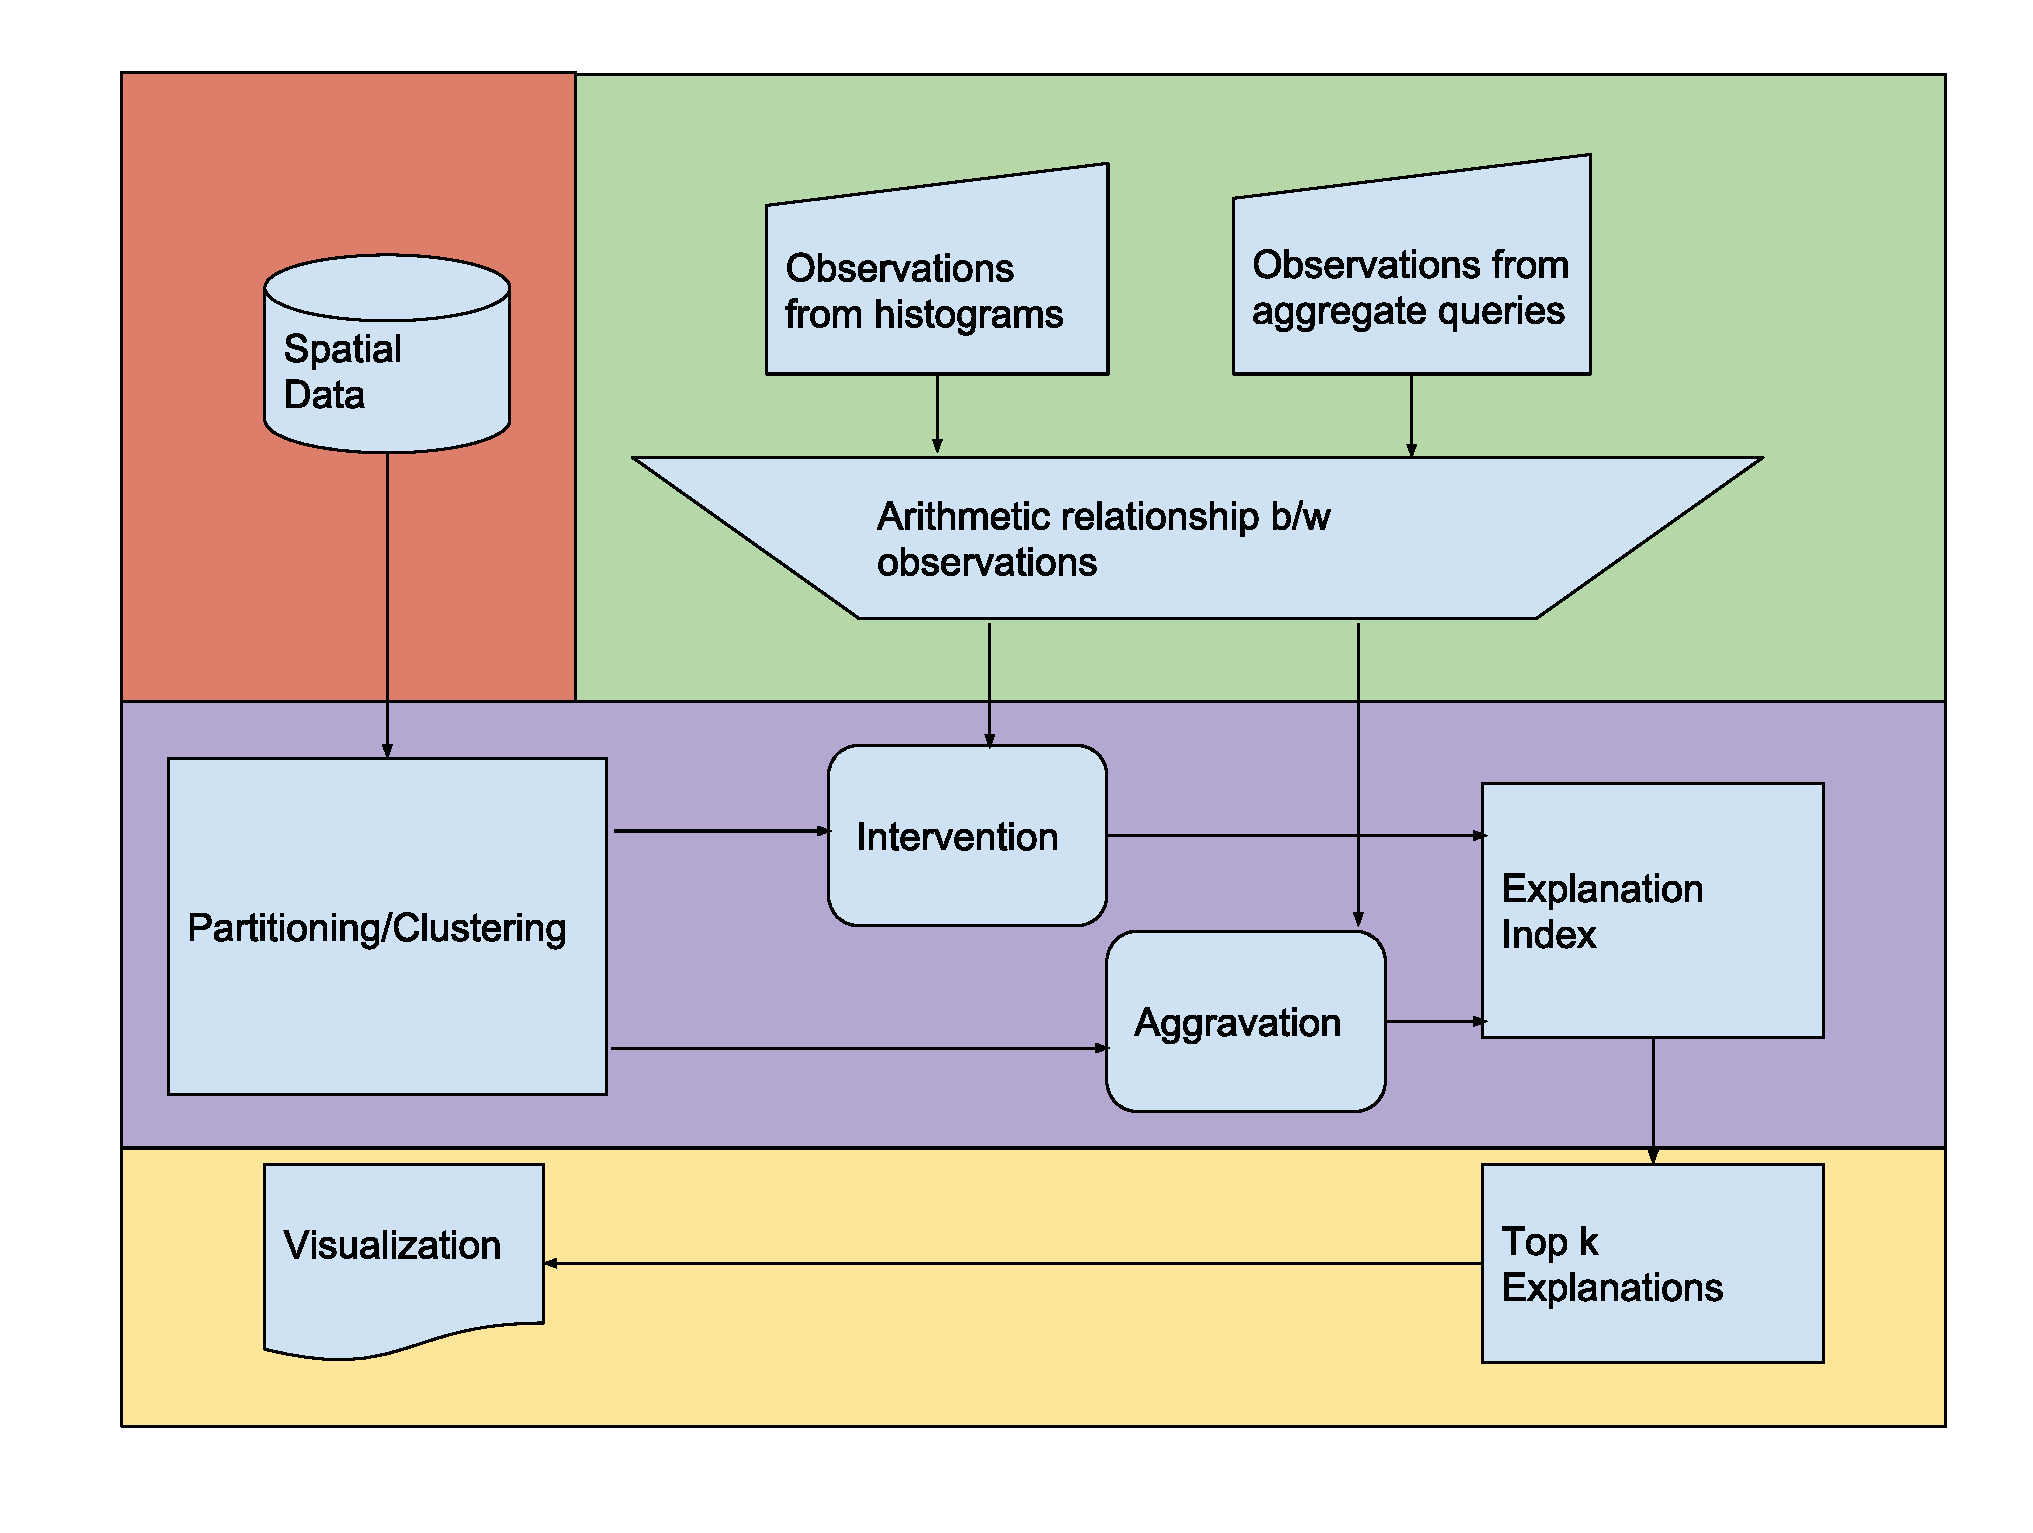
\includegraphics[width=\columnwidth]{framework}
\caption{An outline for our system framework}
\label{fig:framework}
\end{figure}

We created an interface for the system that we have proposed. This interface is web based. It consists of a backend server and a front end for visualizations. The Backend is responsible for querying the Apache Spark daemon with relevant queries. The front end allows the user to define observations and visualize explanations. The front end interface makes use of Mapbox to display the map, Deck.gl to create a visualization overlay on the map. The overlay can be points or polygons. In order to handle state changes in the front end, we used React.js front end library. We also show histograms related to the data. For displaying these histograms, Baidu eCharts library was used. Since the front end was programmed in ES6, webpack was used for transpilation\citep{webpack}. Fig.~\ref{fig:framework} shows us a flow diagram for our system.

In order for the users to easily form observations, our frontend provides them with a series of histograms. Each bar on a histogram represents an aggregate query. Instead of writing queries, the user can easily use the bars in the histograms to be used as variables. These variables can then be used in an arithmetic expression representing the users observations. The user can also define custom variables in the form of aggregate SQL queries manually using the interface.

The back end of the system is an Apache Spark application which calls the Spark daemon for requests of aggravation, intervention, and hierarchical intervention. I must be noted however that there are some operations that the backend performs which are not executed as Spark tasks, such as the creation of an R-Tree. The framework that we have designed requires us to parse and alter queries at multiple points in the pipeline. In order to avoid redesigning the wheel we use the parser implementation provided by PrestoDB\citep{prestodb}.

To allow the front end to communicate with the backend, there is a middleware application. The job of the middleware is to take the input from the front end and execute our backend application with the appropriate function and input parameters. Our middleware is designed using Node js\citep{tilkov2010node,cantelon2017node}. It takes aggregate queries, selectivity range and number of explanations as input and sends it to the backend application. The results are then sent to the frontend.

\begin{figure}[h]
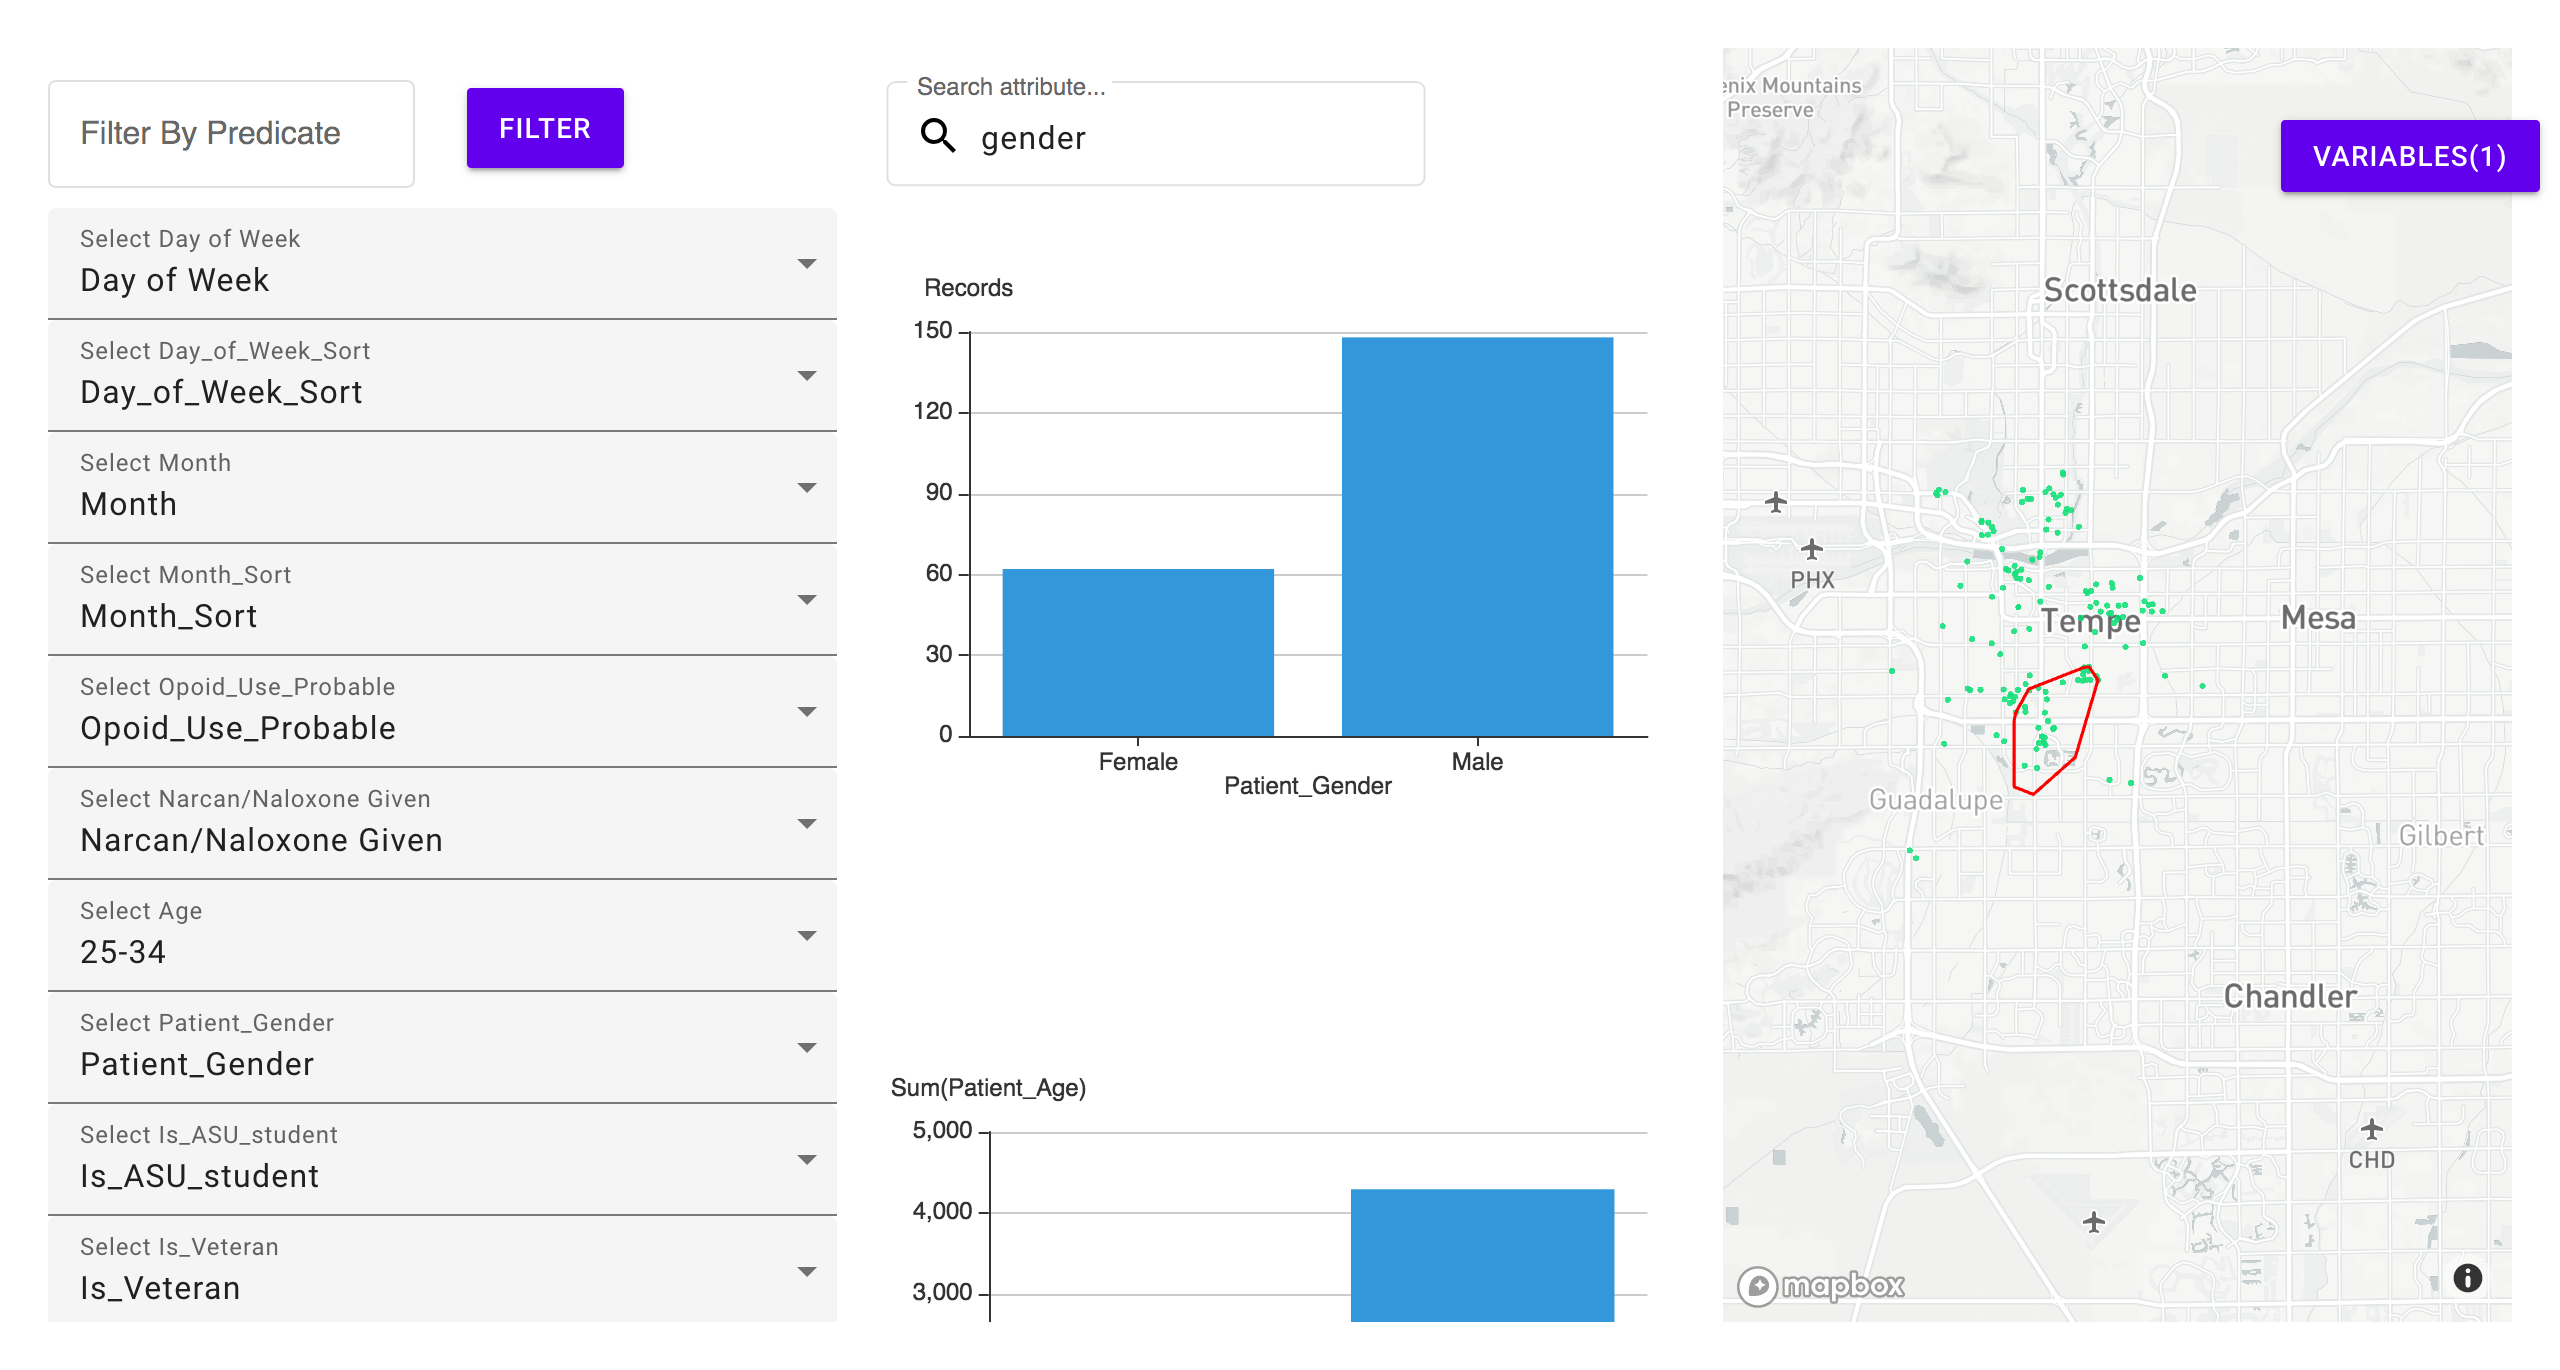
\includegraphics[width=\columnwidth]{interface.png}
\caption{The web interface for our solution}
\label{fig:interface}
\end{figure}

Fig.~\ref{fig:interface} shows the interface that we have created for our solution. The users may add variables from the histograms or they may add them from their own sql queries. The interface allows the user to filter by attribute before viewing the histograms.

\chapter{EXPERIMENTS/EVALUATION}
\label{chp:eval}
\label{sec:evaluation}
%Why we need evaluation\label{sec:relevance}
The main contribution of this thesis is to introduce a new approach for explanations(Hierarchical Intervention). We evaluate this new approach in a number of different ways. We perform qualitative evaluation and speed/scalability evaluation.

In order to compare the different clustering techniques that we use in hierarchical intervention, we did a couple of experiments. Our solution relies on the fact that the higher the influence or intensity are a measure of the value of our explanations. We used a number of observations on the NYC TLC data to see how each clustering technique fares against the others.

\textbf{Experimental Setup}. In order to compare the different spatial partitioning techniques, we set up an environment for experiments. Since the quality of the explanations does not depend on the speed and scale of the system, these experiments were performed on a single node machine with an i7 6400 3.5 GHz CPU and 8GB of RAM. The dataset used for this experiment was the NYC TLC data for January 2016. This data contains ~10 million trips.

We found that R-Tree and R* Tree partitioning is usually more stable than K Means or Greedy Clustering. The stability of the clustering technique is referring to its monotonicity of the explanation as a function of the number of clusters. Fig.~\ref{fig:hieint_passenger_count} shows the influence against the number of clusters where the observation is the average passenger count. The influence and intensity are closer to a sinusoidal curve than a exponential or logarithmic curve. Fig.~\ref{fig:clustering_comparison} shows another observation and a plot of the influence of R-Tree and R*-Tree as well. The influence as a function of the number of clusters is a lot more monotonic here. Furthermore, R* Tree has a higher influence on average compared to other approaches making it a lot more suitable for explanations.
%Reasons for selecting evaluation criteria
The qualitative evaluation that we define is based on K-Folds cross validation. The reason for selecting these evaluations is to measure how the top explanations provided by each approach fair as stand alone parts of data as well as their effects on the entire dataset as a whole. Other than qualitative analysis we look at the speed and scalability of each approach for performance evaluation.

\begin{figure}[H]
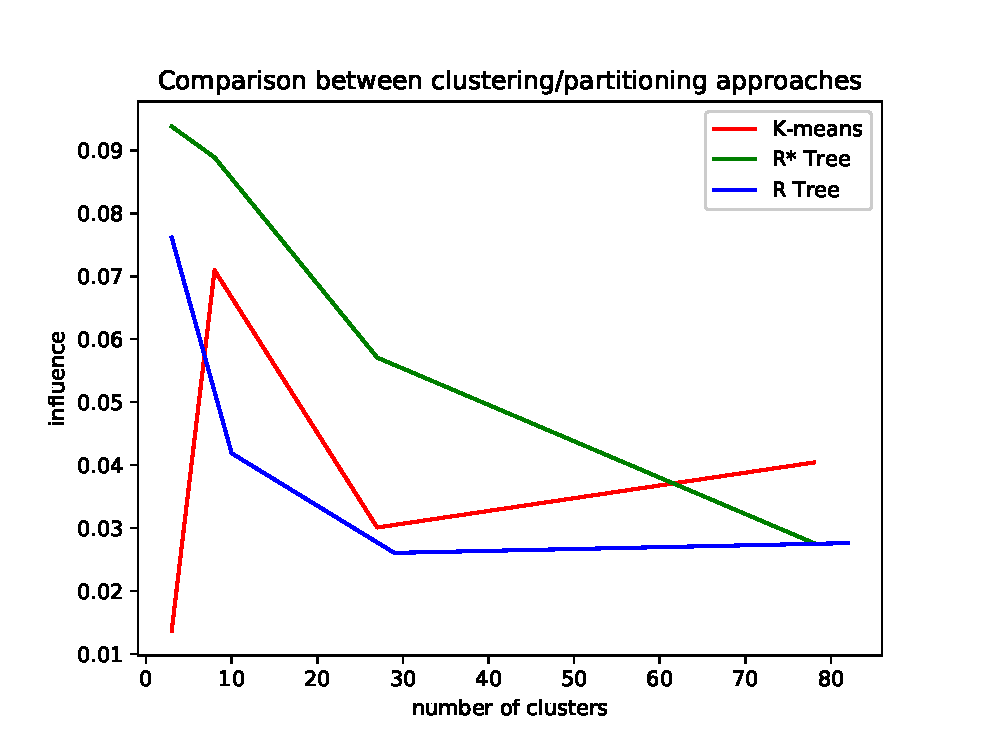
\includegraphics[width=\columnwidth]{clustering_comparison}
\caption{Comparison of Influence against number of clusters for K-Means, R-Tree and R*-Tree}
\label{fig:clustering_comparison}
\end{figure}

\begin{figure}[h]
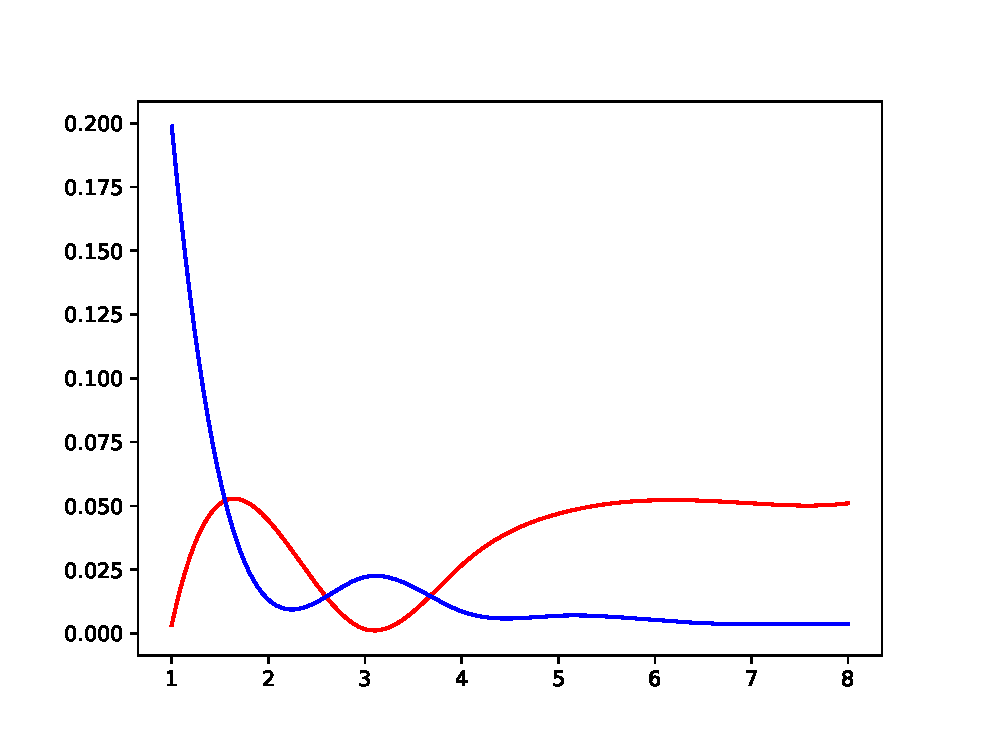
\includegraphics[width=\columnwidth]{hieint_passenger_count}
\caption{Comparison of Influence and Intensity against level of hierarchy with average passenger count as observation}
\label{fig:hieint_passenger_count}
\end{figure}
%How does each approach compare
\textbf{Influence Comparison.}
\begin{figure}[h]
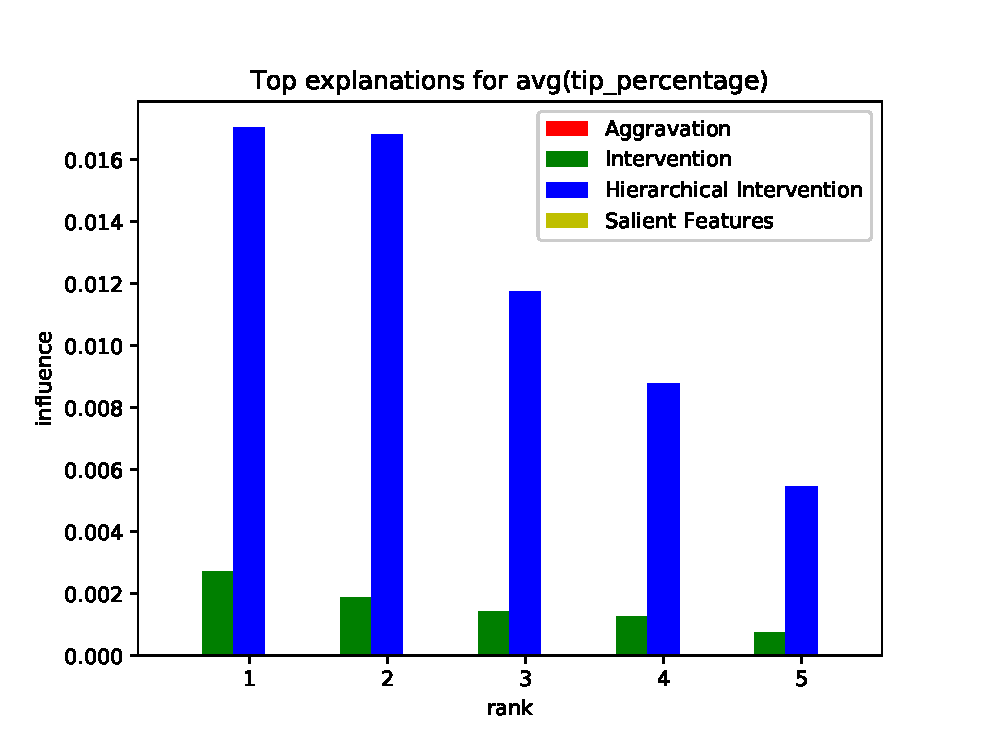
\includegraphics[width=\columnwidth]{Top_explanations_for_avg_tip_percentage_influence}
\caption{Influence for Spatial explanation for average tip percentage(Lower is better)}
\label{fig:influence_comparison}
\end{figure}

Fig.~\ref{fig:influence_comparison} shows the comparison between the influence of different approaches. Salient features and Aggravation have a very low influence compared to Intervention and hierarchical intervention. This is because the explanations provided by those approaches cover a very small portion of the entire dataset. This makes removing the associated data have a negligible impact on the entire data.

\section{K-Folds cross validation}
In order to qualitatively assess the solutions, we use K-Folds cross validation\citep{refaeilzadeh2009cross}. Since we do not have ground truth for our explanations, we have to make a compromise in terms of estimating how good our solution is. Our assumption here is that in general, a good explanation would stand out on unseen data i.e. given a good explanation on part of the data, it would give similar results on unseen parts of the data. This is the same assumption that was made by \cite{chirigati2016data} in their evaluation of the Data Polygamy framework. We split the data into $k$ parts. The data was divides by the month of the year. This is because there are specific observable patterns in each month, e.g. weekends have less density of trips than the weekdays for the dataset we evaluated. One of the parts is used to find the explanation(the training data). The rest of the data is the test data. We also calculate an explanation of the test data. The relative distance between the explanation index of the test data and the explanation index of the explanation provided by the training data when applied to the test data is used as a measure of evaluation.

The reason for using K-Folds evaluation in this way is because there is a lack of data with the ground truth values. We can see similar approaches for evaluation used in the works that our approach has been inspired from. The evaluation in the work by \cite{roy2014formal} is less relaxed because they only look at the magnitude of intervention for evaluation, whereas, \cite{chirigati2016data} also use the NYC TLC data for evaluation using the assumption that the data for 2011 and 2012 have the same pattern. In order to measure the quality of the explanations provided by hierarchical intervention we compare it with intervention and aggravation.

There is a reason for applying the explanation provided by the training data to the test data. The observation can be anything. The size of the training and test data is different depending on $k$. The observation can depend on the size of the data. This adds a bias when the explanation index for the training data is compared with the explanation index of the test data. Thus, we must apply the explanation provided by the training data on the test data and compare it with the explanation when we apply the same approach to the test data.

\begin{figure}[h]
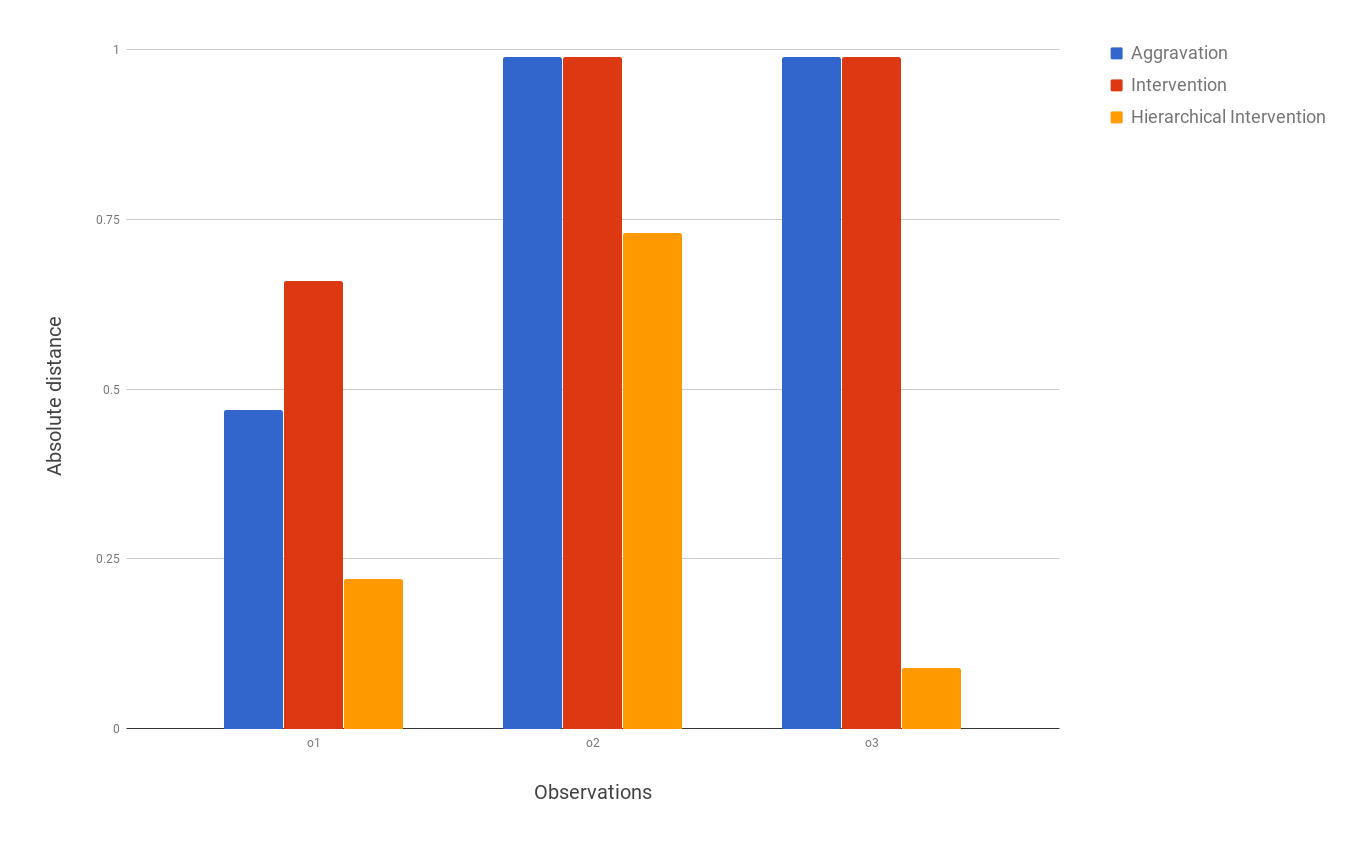
\includegraphics[width=\columnwidth]{kfolds.png}
\caption{The result for k-folds evaluation shows good results when the approach is used in favor of influence(lower is better) for observations represented by Queries~\ref{qry:o1},~\ref{qry:o2}, and ~\ref{qry:o3}}
\label{fig:kfolds}
\end{figure}

\textbf{Experimental Setup}. We performed the evaluation on the first 5 months of data from the NYC yellow cab dataset from 2016. The data spanned ~ 50 million trips. The $k$ for our evaluation was $5$. This value was chosen after a series of experiments. We wanted the size of each partition to be large enough to support our generalization assumption. If the solution space for evaluation is small, it leads to inconsistent results. Each month represented a partition for k-folds evaluation. According to our analysis, we found that the approach works very well with low values of alpha. Fig.~\ref{fig:kfolds} shows some of the results of our evaluation for a number of observations. The lower the value of the relative distance, the better the results.

The relative distance in the K Folds cross validation represents how much the explanation impact changes when we look at the explanations in the context of unseen data. A relative distance of zero represents that the explanation has the same impact on unseen data as if we had seen the data. A relative distance of one would represent that the top explanation for the unseen data has nothing in common with the explanation of seen data. Let $e_{test}$ be the explanation index for the test set. Let $e_{train}$ be the explanation index for the training set. Then,

$$relative\_distance = \frac{|e_{test}-e_{train}|}{|e_{test}+e_{train}|}$$

The relative distance metric was chosen because of its nature of showing a steep decline when two solutions do not match. It is also ideal because it caters to the different types of observations that a user can specify. Since the observations in our system are defined as an arithmetic operation over aggregate queries, they do not have bounds on their values. Thus, it makes relative distance a useful metric for measuring similarity.

Here are the observations that we show in Fig.~\ref{fig:kfolds}:
\renewcommand{\lstlistingname}{Query}% Listing -> Algorithm
\begin{lstlisting}[language=SQL, caption=o1 for Fig.~\ref{fig:kfolds}, label=qry:o1]
Select count(*) as q1 from data where payment_type=1;
Select count(*) as q2 from data where payment_type=2;
Observation = q1/q2
\end{lstlisting}

\begin{lstlisting}[language=SQL, caption=o2 for Fig.~\ref{fig:kfolds}, label=qry:o2]
Select AVG(trip_distance) as q1 where passenger_count=4;
Observation = q1
\end{lstlisting}

\begin{lstlisting}[language=SQL, caption=o3 for Fig.~\ref{fig:kfolds}, label=qry:o3]
Select count(*) as q1 from data where vendorid=1;
Select count(*) as q2 from data where vendorid=2;
Observation = q1/q2
\end{lstlisting}

\section{Precision and Recall}
\begin{wrapfigure}{R}{0.4\textwidth}
  \begin{center}
    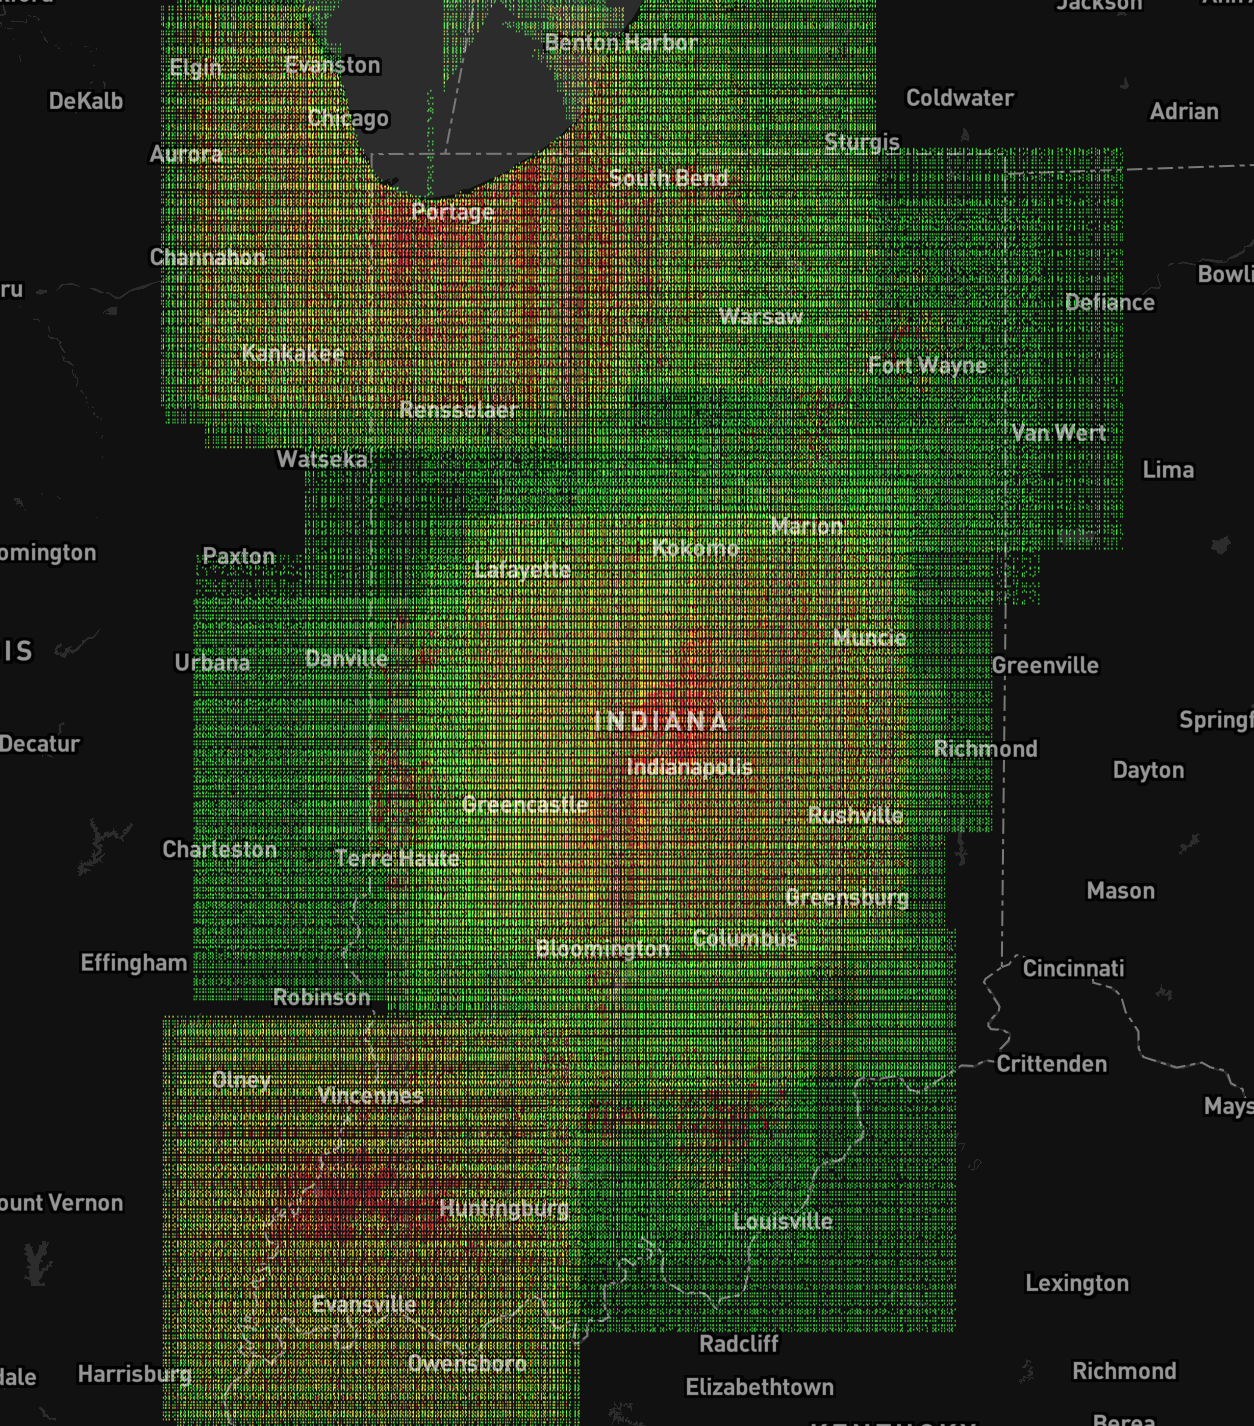
\includegraphics[width=0.38\textwidth]{outbreakheatmap.png}
  \end{center}
  \caption{A heatmap showing sythesized data}
  \label{fig:synthesized_data}
\end{wrapfigure}
% \begin{figure}[h]
% 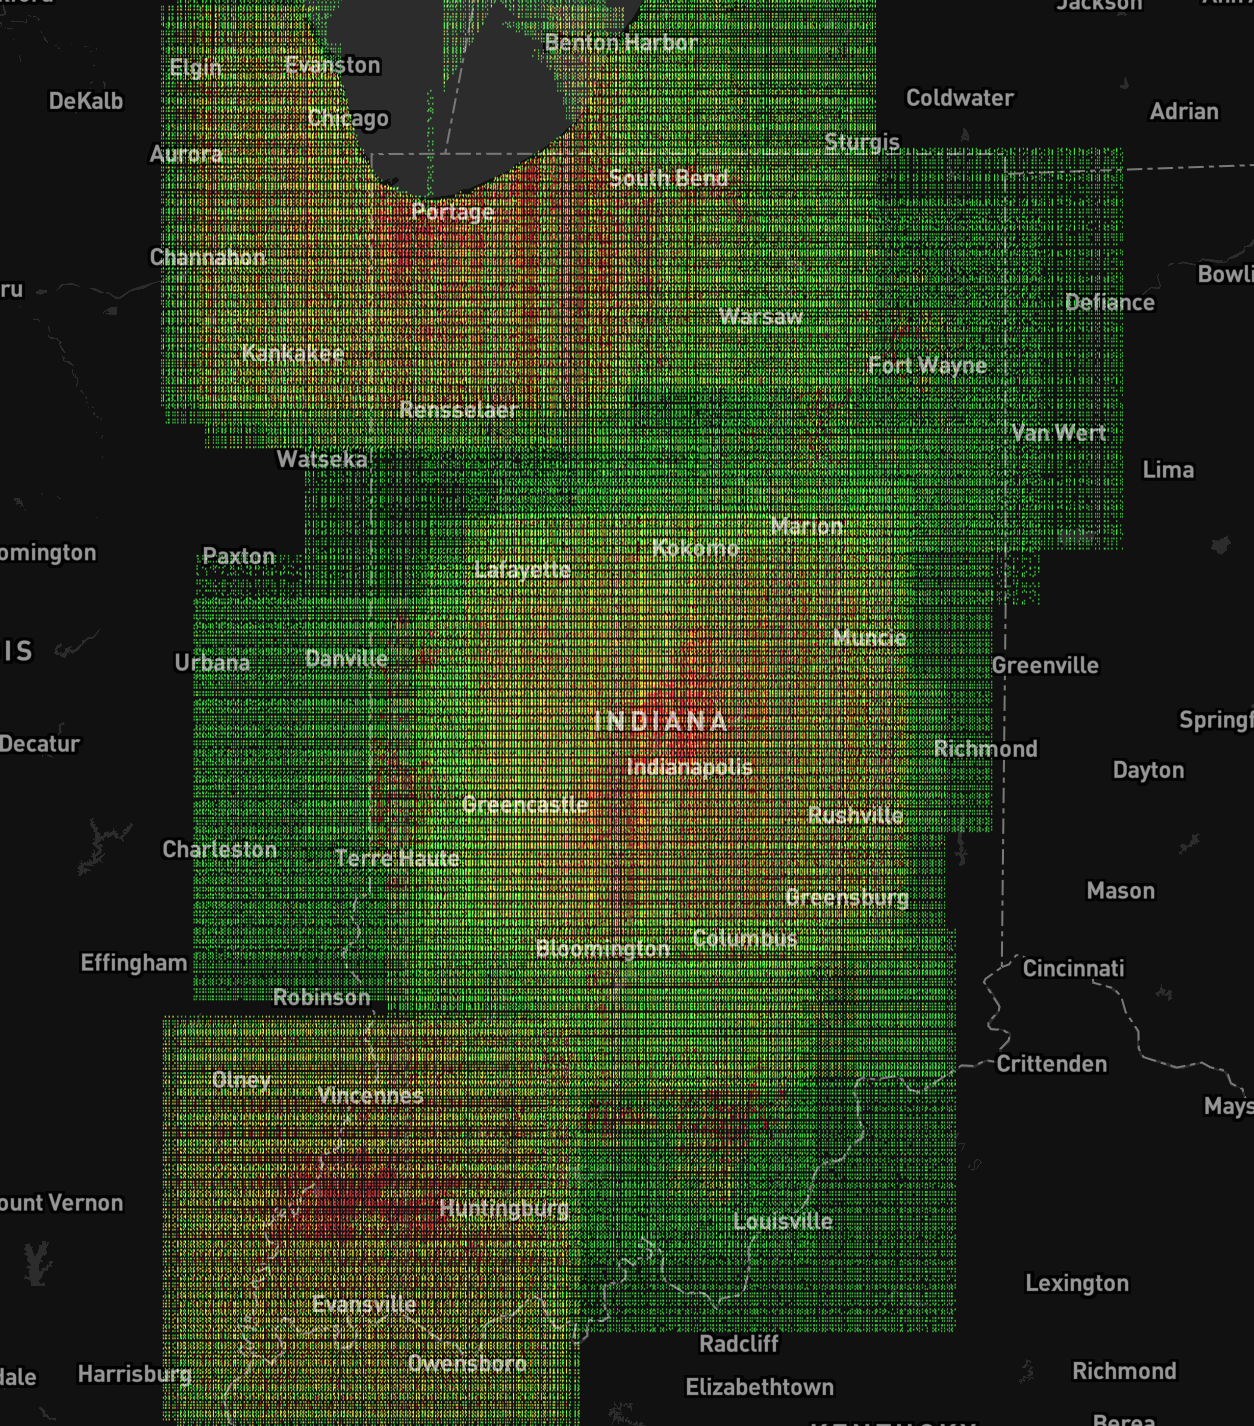
\includegraphics[width=\columnwidth]{outbreakheatmap.png}
% \caption{A heatmap showing sythesized data}
% \label{fig:synthesized_data}
% \end{figure}

Since it is very difficult to find datasets with the ground truth we used synthetic datasets to evaluate our solution\citep{maciejewski2009generating}. The synthetic dataset is fabricated using real data from Indiana Public Health Emergency Surveillance System. This data contains information about Patients in Indiana and their health issues over time and location. We can calculate precision and recall using this data\citep{powers2011evaluation}. The data is synthesized in such a way that it shows similar patterns to the actual data. Synthetic data related to outbreaks of certain diseases is synthesized into this data. In order to evaluate our system, we used the temporal component of the outbreak and the type of disease as our observation. To be specific, the synthetic data consisted of an outbreak of Gastrointestinal infection in July. Our observation was the ratio of the number of gastrointestinal infection incidents between June and July when there's an infection against the number of gastrointestinal infection incidents between June and July in synthesized data where there wasn't an outbreak. Precision and Recall was calculated by comparing the areas of the top ten explanations related to the ground truth with the approximate area covered by the outbreak data. We cannot use the individual points to calculate precision and recall because there is a lot of data unrelated to the outbreak which occurs in proximity. To put things into context, each instance of the synthesized data contains ~2 million records. The data related to the outbreak consists of a few dozen records. Fig.~\ref{fig:synthesized_data} shows a heatmap of all the points in the synthesized data. The outbreak for this particular instance only affects a small part of Indiana to the North West just below Lake Michigan. Fig.~\ref{fig:precisionrecall} shows the points representing the outbreak as well as some of the top polygons returned using Hierarchical Intervention. While our system is designed to work fast on partitioning techniques with no overlaps like K-Means and Greedy Hierarchical Clustering. Some of the clustering apporaches that we use which give better results do have overlaps. Thus we used R*-Tree partitioning in our example. The candidate explanations provided by this partitioning techniques can have spatial overlaps.


% \begin{wrapfigure}{R}{0.5\textwidth}
%   \begin{center}
%     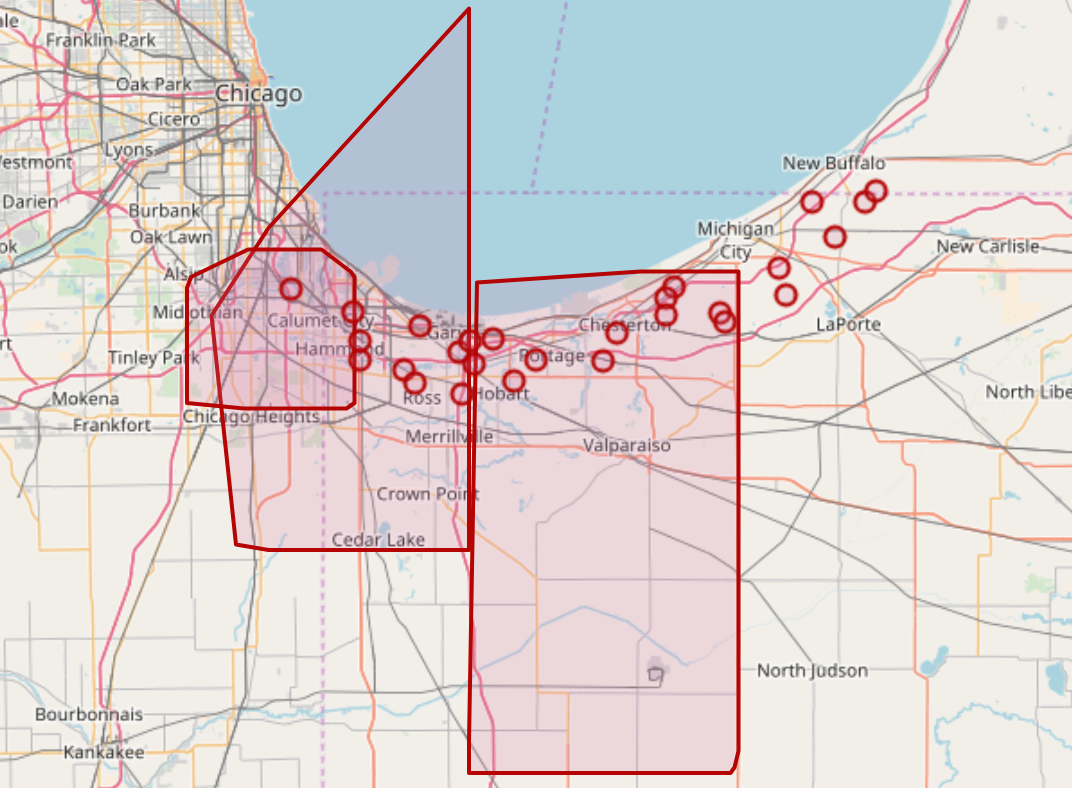
\includegraphics[width=0.48\textwidth]{precisionrecall.png}
%   \end{center}
%   \caption{Synthetic Outbreak data. The circles show the ground truth while the polygons show the relevant explanations produced by our system}
%   \label{fig:precisionrecall}
% \end{wrapfigure}
\begin{figure}[h]
\begin{center}
  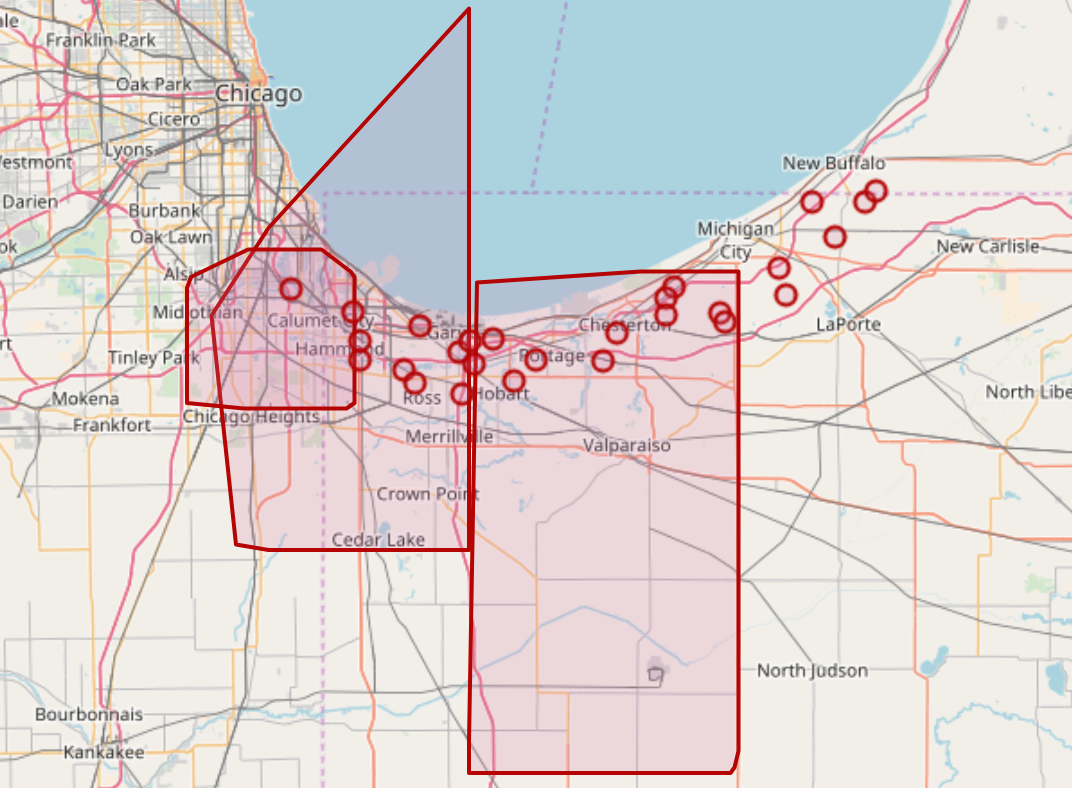
\includegraphics[width=0.7\columnwidth]{precisionrecall.png}
\end{center}
\caption{Synthetic Outbreak data. The circles show the ground truth while the polygons show the relevant explanations produced by our system}
\label{fig:precisionrecall}
\end{figure}

Let $E$ be the area represented by our polygons. Let $O$ be the area represented by the Outbreak points. Then,
$$Precision = \frac{E \cap O}{E} = 0.31$$
\newpage
For calculating recall, we can use the actual outbreak points since it doesn't require false positives.
$$Recall = \frac{true\_positives}{false\_negatives} = 0.74$$




\subsection{Comparison}
We compared the precision and recall of Hierarchical Intervention with Aggravation and Intervention.
\\
\textbf{Aggravation}. We used the same observation for aggravation that we did for Hierarchical Intervention. From the top ten explanations, only one of the explanation was able to predict one of the 27 correct tuples in the ground truth.
$$Precision = 0.01$$
$$Recall = 0.04$$


\textbf{Intervention}. Finally, Intervention was used to find an explanation. Since there was only one hospital in the area of the outbreak, Intervention was able to provide that hospital as a relevant predicate in an explanation. This resulted in all the ground truth points being included in the explanation! However, since there are a large number of tuples related to this predicate, it resulted in a low precision.

$$Precision = 0.0003,\ Recall = 1$$


% \begin{wrapfigure}{r}{0.5\textwidth}
%   \begin{center}
%     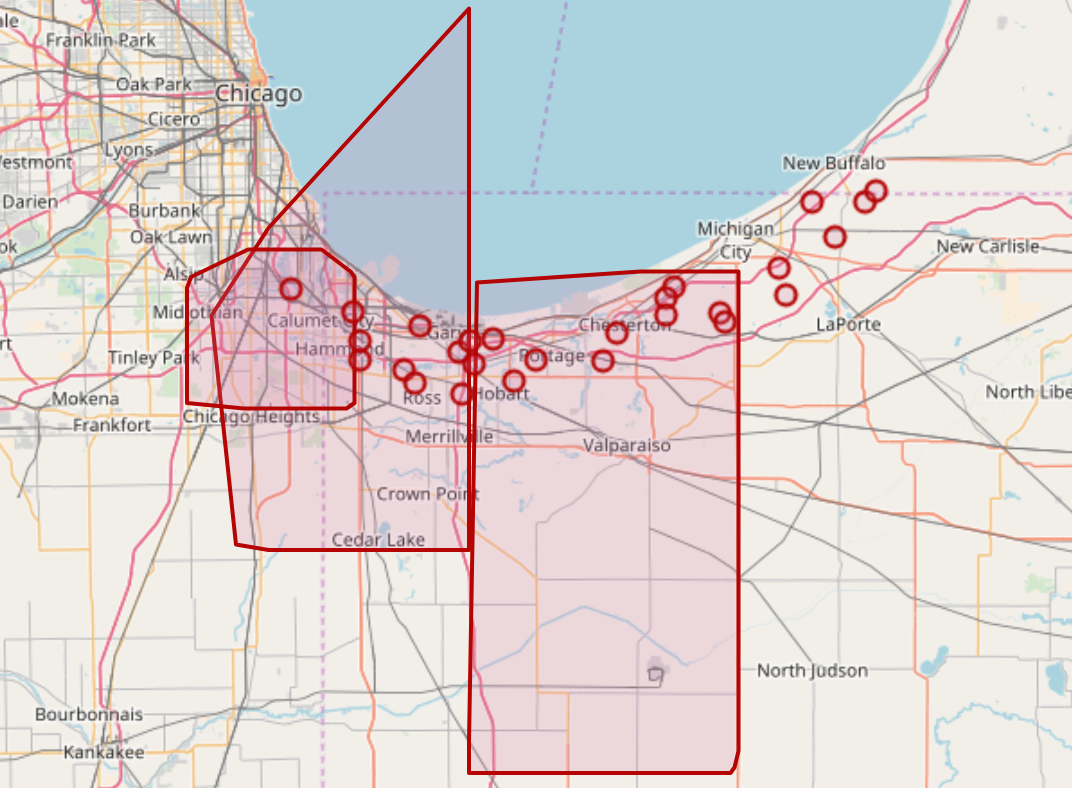
\includegraphics[width=0.48\textwidth]{precisionrecall.png}
%   \end{center}
%   \caption{Synthetic Outbreak data. The circles show the ground truth while the polygons show the relevant explanations produced by our system}
% \label{fig:spatial_spatial_vertical}
% \end{wrapfigure}



% \textbf{Influence and Intensity for Hierarchical Intervention}
% \begin{figure}[H]
% 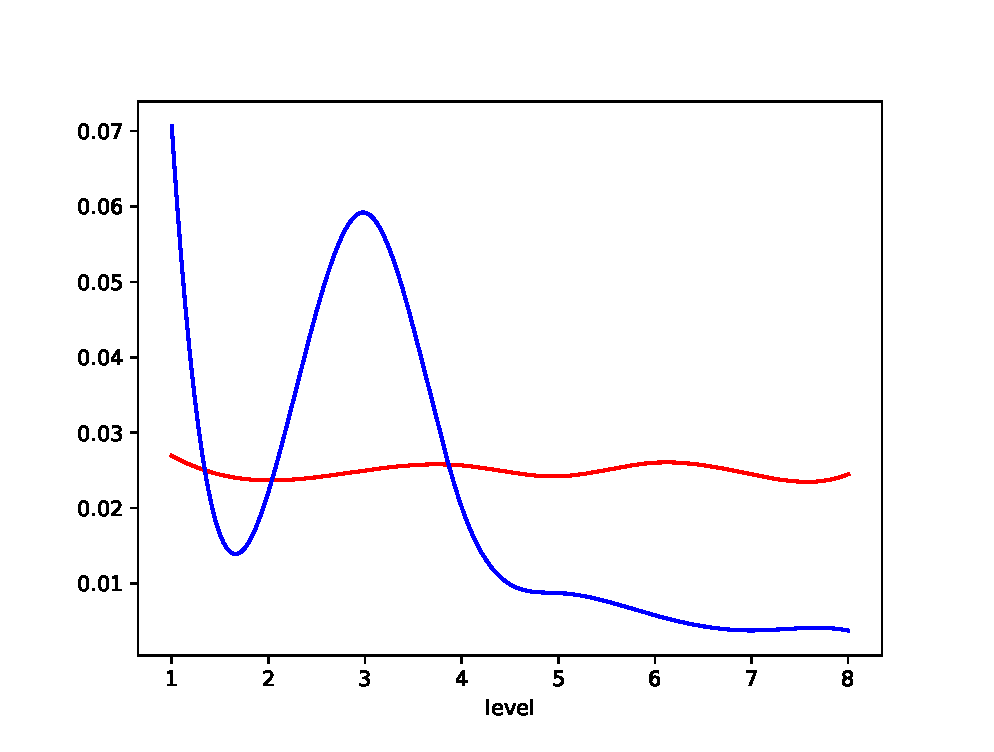
\includegraphics[width=\columnwidth]{heiint_tip_percentage}
% \caption{Comparison of Influence and Intensity against level of hierarchy with average tip percentage as observation}
% \label{fig:hieint_tip_percentage}
% \end{figure}




% \begin{figure}[H]
% 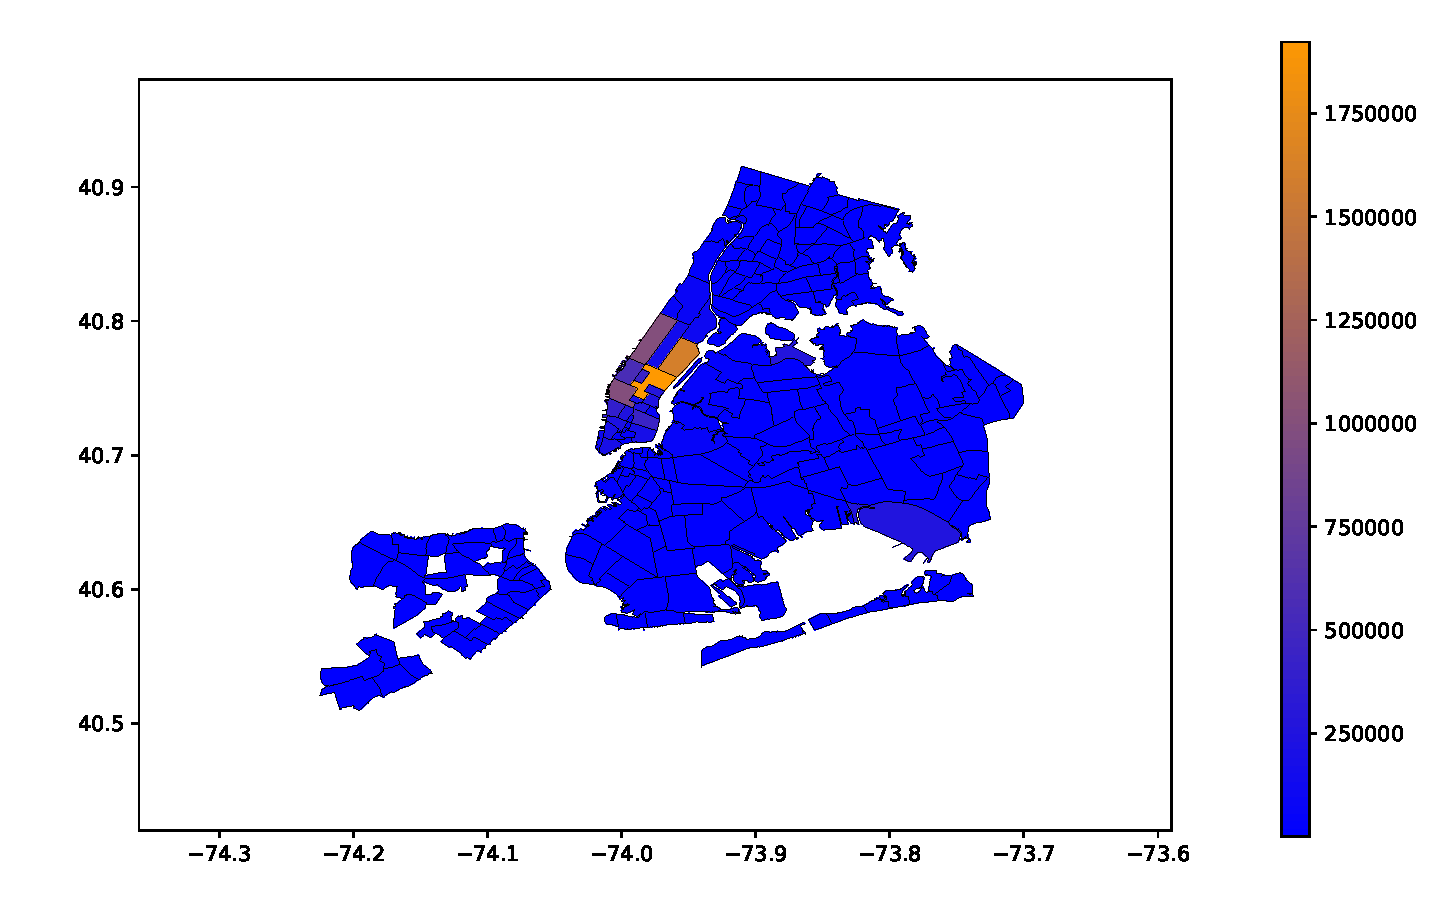
\includegraphics[width=\columnwidth]{count_initial}
% \caption{The number of trips for each zone by pickup zone}
% \label{fig:count_initial}
% \end{figure}

% \begin{figure}[H]
% 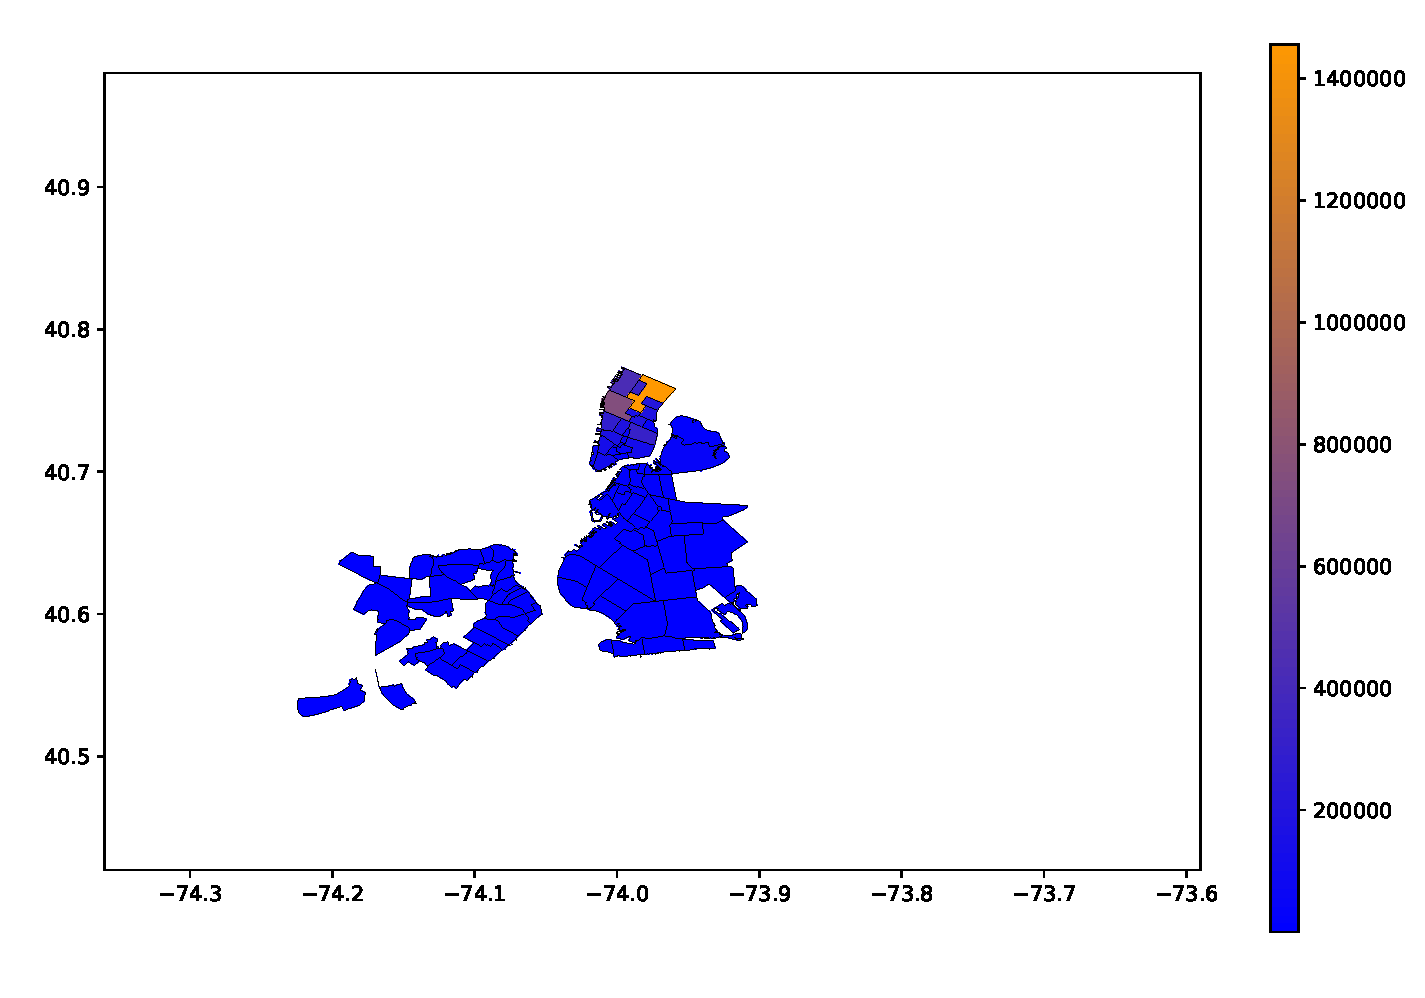
\includegraphics[width=\columnwidth]{top_level_2}
% \caption{Number of rows that represent the top explanation for average tip percentage at level 2}
% \label{fig:top_level_2}
% \end{figure}

% \begin{figure}[H]
% 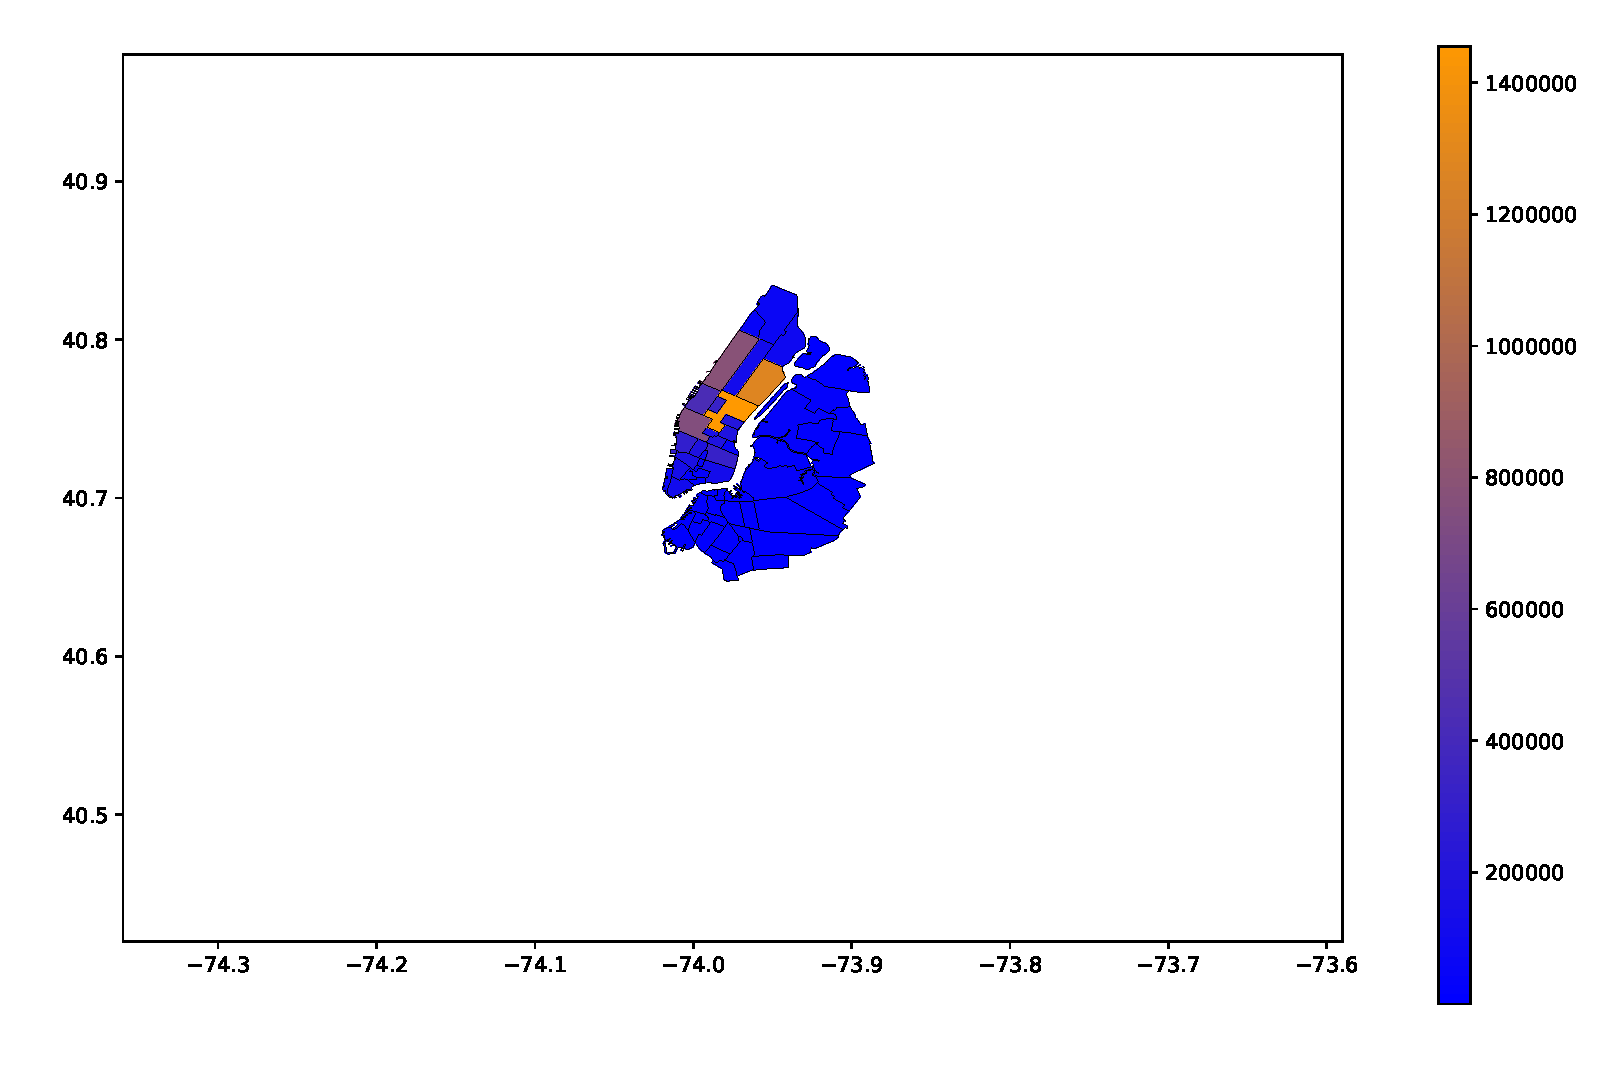
\includegraphics[width=\columnwidth]{top_level_3}
% \caption{Number of rows that represent the top explanation for average tip percentage at level 3}
% \label{fig:top_level_3}
% \end{figure}

% \begin{figure}[H]
% 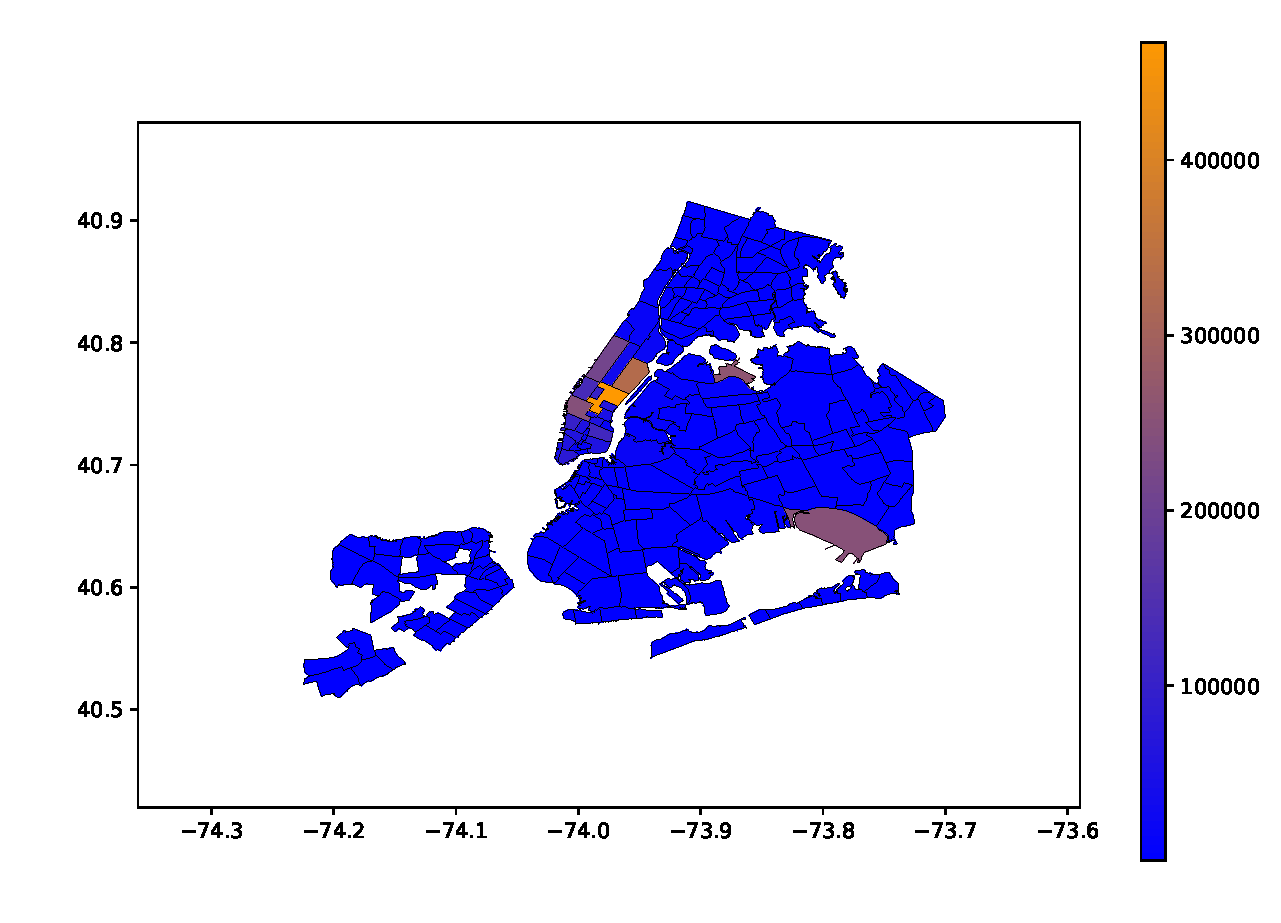
\includegraphics[width=\columnwidth]{level_3_removed}
% \caption{The cartogram for the data when we remove he level 3 explanation}
% \label{fig:level_3_removed}
% \end{figure}


\section{Speed and Scalability}
\label{sec:speed}
The speed of each approach is simply the time taken to calculate the explanations. The time varies depending on the size of the data. For performance evaluation, we used the NYC TLC data for 2016. The data is divided into months. As we increase the number of months to be processed, the time taken for each approach increases almost linearly for aggravation, intervention and hierarchical intervention. For salient features, the time increases slightly exponentially. The results of our evaluation are displayed in Fig.~\ref{fig:performance}

\textbf{Experimental Setup}. The speed of each approach is simply the time taken to calculate the explanations. Since all the approaches are implemented on top of distributed systems, the time varies depending on the number of nodes used. We experimented with calculating explanations for 1,3, and 5 months in a distributed environment. For the cluster, we used Google Compute Engine nodes(1 vCPU, 3.5GB RAM, 4 nodes). All the nodes in our cluster had the same specifications. The Aggravation, Intervention and Hierarchical Intervention were tested on Apache Spark running on YARN while the Salient Features were generated with the Data Polygamy Framework running on YARN.
\begin{figure}[h]
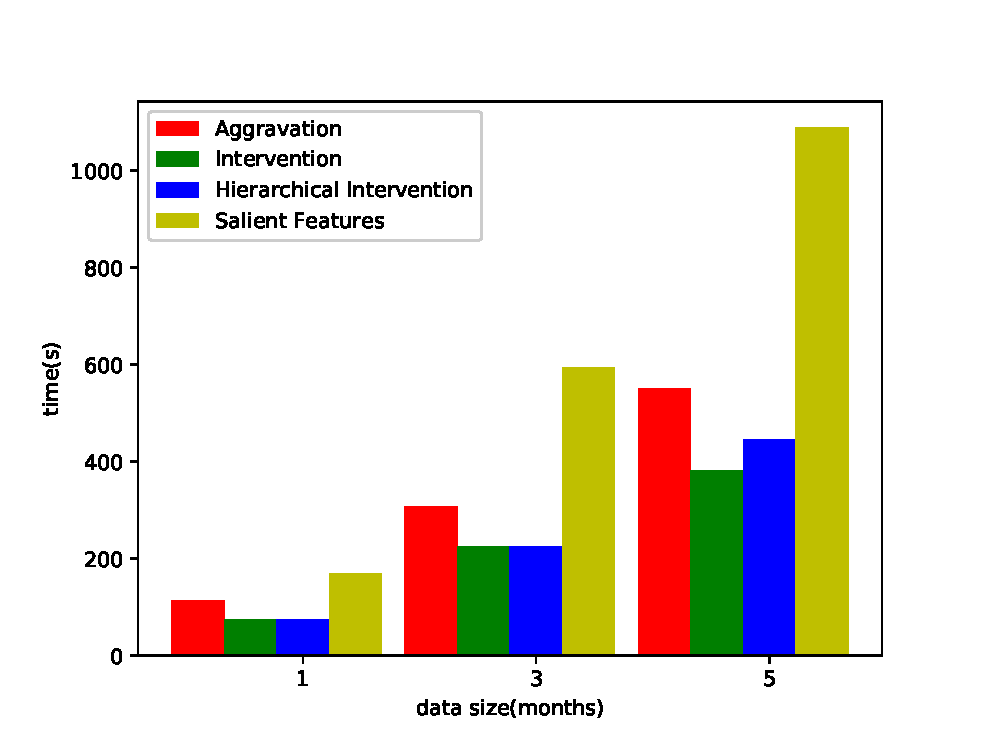
\includegraphics[width=\columnwidth]{performance}
\caption{Time taken by each approach as we increase the size of data}
\label{fig:performance}
\end{figure}
\newline
The run times that were observed can be explained as follows. Aggravation takes the least amount of time of the compared approaches. Intervention costs more than aggravation because it includes the additional step of calculating statistics for the attributes as well as iterating the table. Hierarchical Intervention takes more time than aggravation but less time than intervention. This is because of several factors. One of the factors is that when we are using intervention and aggravation, we are using several attributes, on the other hand, hierarchical intervention only uses the spatial attribute. On the other hand, we are creating a hierarchy. The in the case of this analysis we only used one query as the observation for the sake of comparison. However, multiple queries can affect the comparison as well. The time taken by Salient Features is also affected by a number of factors. First, the implementation of the salient features that we use is the one used in the Data Polygamy Framework \citep{chirigati2016data}. This approach uses the MapReduce framework. The other approaches use the Spark framework. Since Spark makes use of an execution plan which is more efficient than MapReduce, it is a factor in the slower runtime of the Salient Features approach. Thus, when comparing salient features to the other approaches, this can be considered something similar to black box testing. The most expensive computation step in salient features is the interpolation step which doesn't occur in the other approaches.


% \begin{figure}[H]
% 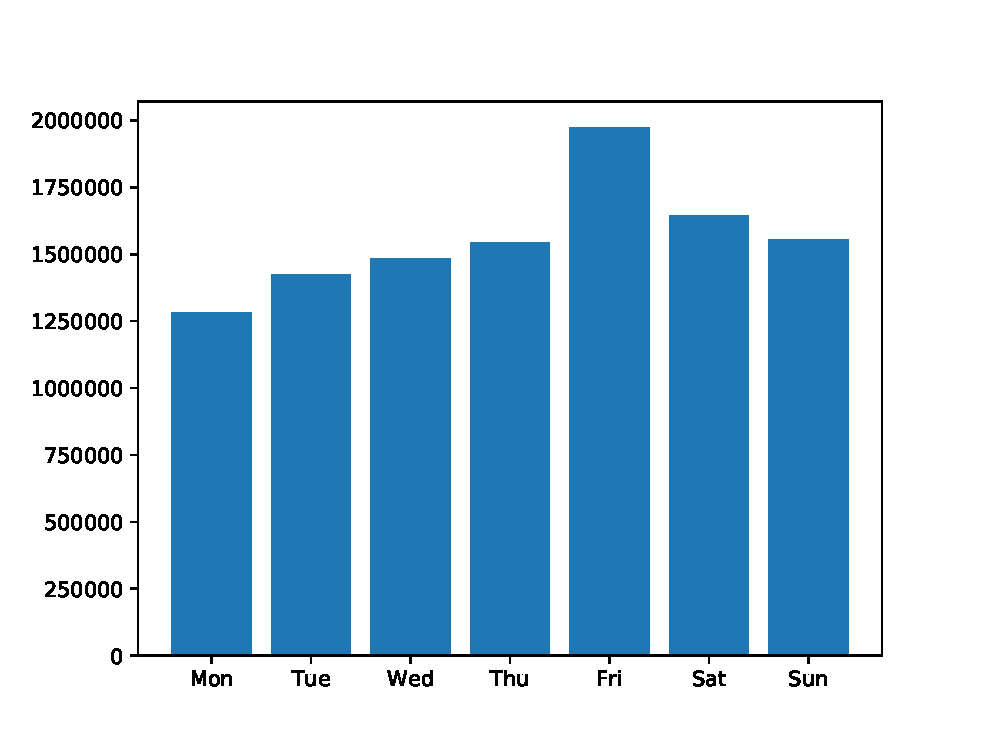
\includegraphics[width=\columnwidth]{day_comparison}
% \caption{Number of trips against trip day}
% \label{fig:day_comparison}
% \end{figure}

\chapter{Conclusion}
We looked at different approaches for spatial explanations for arbitrary observations. We found that Hierarchical Intervention is a great way to explain spatial data as it outperforms other approaches in most of the evaluation metrics. Our system is designed to 
%-----------------------back matter
{\singlespace
% Making the references a "part" rather than a chapter gets it indented at
% level -1 according to the chart: top of page 4 of the document at
% ftp://tug.ctan.org/pub/tex-archive/macros/latex/contrib/tocloft/tocloft.pdf
\addcontentsline{toc}{part}{REFERENCES}
\bibliographystyle{asudis}
\bibliography{dis}}
\renewcommand{\chaptername}{APPENDIX}
\addtocontents{toc}{APPENDIX \par}
\appendix
\chapter{RAW DATA}

\include{vita}
\end{document}
